\documentclass[twoside]{book}

% Packages required by doxygen
\usepackage{fixltx2e}
\usepackage{calc}
\usepackage{doxygen}
\usepackage{graphicx}
\usepackage[utf8]{inputenc}
\usepackage{makeidx}
\usepackage{multicol}
\usepackage{multirow}
\PassOptionsToPackage{warn}{textcomp}
\usepackage{textcomp}
\usepackage[nointegrals]{wasysym}
\usepackage[table]{xcolor}

% NLS support packages
\usepackage[french]{babel}

% Font selection
\usepackage[T1]{fontenc}
\usepackage{mathptmx}
\usepackage[scaled=.90]{helvet}
\usepackage{courier}
\usepackage{amssymb}
\usepackage{sectsty}
\renewcommand{\familydefault}{\sfdefault}
\allsectionsfont{%
  \fontseries{bc}\selectfont%
  \color{darkgray}%
}
\renewcommand{\DoxyLabelFont}{%
  \fontseries{bc}\selectfont%
  \color{darkgray}%
}
\newcommand{\+}{\discretionary{\mbox{\scriptsize$\hookleftarrow$}}{}{}}

% Page & text layout
\usepackage{geometry}
\geometry{%
  a4paper,%
  top=2.5cm,%
  bottom=2.5cm,%
  left=2.5cm,%
  right=2.5cm%
}
\tolerance=750
\hfuzz=15pt
\hbadness=750
\setlength{\emergencystretch}{15pt}
\setlength{\parindent}{0cm}
\setlength{\parskip}{0.2cm}
\makeatletter
\renewcommand{\paragraph}{%
  \@startsection{paragraph}{4}{0ex}{-1.0ex}{1.0ex}{%
    \normalfont\normalsize\bfseries\SS@parafont%
  }%
}
\renewcommand{\subparagraph}{%
  \@startsection{subparagraph}{5}{0ex}{-1.0ex}{1.0ex}{%
    \normalfont\normalsize\bfseries\SS@subparafont%
  }%
}
\makeatother

% Headers & footers
\usepackage{fancyhdr}
\pagestyle{fancyplain}
\fancyhead[LE]{\fancyplain{}{\bfseries\thepage}}
\fancyhead[CE]{\fancyplain{}{}}
\fancyhead[RE]{\fancyplain{}{\bfseries\leftmark}}
\fancyhead[LO]{\fancyplain{}{\bfseries\rightmark}}
\fancyhead[CO]{\fancyplain{}{}}
\fancyhead[RO]{\fancyplain{}{\bfseries\thepage}}
\fancyfoot[LE]{\fancyplain{}{}}
\fancyfoot[CE]{\fancyplain{}{}}
\fancyfoot[RE]{\fancyplain{}{\bfseries\scriptsize Généré le Jeudi 12 Octobre 2017 11\+:43\+:16 pour My Project par Doxygen }}
\fancyfoot[LO]{\fancyplain{}{\bfseries\scriptsize Généré le Jeudi 12 Octobre 2017 11\+:43\+:16 pour My Project par Doxygen }}
\fancyfoot[CO]{\fancyplain{}{}}
\fancyfoot[RO]{\fancyplain{}{}}
\renewcommand{\footrulewidth}{0.4pt}
\renewcommand{\chaptermark}[1]{%
  \markboth{#1}{}%
}
\renewcommand{\sectionmark}[1]{%
  \markright{\thesection\ #1}%
}

% Indices & bibliography
\usepackage{natbib}
\usepackage[titles]{tocloft}
\setcounter{tocdepth}{3}
\setcounter{secnumdepth}{5}
\makeindex

% Hyperlinks (required, but should be loaded last)
\usepackage{ifpdf}
\ifpdf
  \usepackage[pdftex,pagebackref=true]{hyperref}
\else
  \usepackage[ps2pdf,pagebackref=true]{hyperref}
\fi
\hypersetup{%
  colorlinks=true,%
  linkcolor=blue,%
  citecolor=blue,%
  unicode%
}

% Custom commands
\newcommand{\clearemptydoublepage}{%
  \newpage{\pagestyle{empty}\cleardoublepage}%
}


%===== C O N T E N T S =====

\begin{document}

% Titlepage & ToC
\hypersetup{pageanchor=false,
             bookmarks=true,
             bookmarksnumbered=true,
             pdfencoding=unicode
            }
\pagenumbering{roman}
\begin{titlepage}
\vspace*{7cm}
\begin{center}%
{\Large My Project }\\
\vspace*{1cm}
{\large Généré par Doxygen 1.8.8}\\
\vspace*{0.5cm}
{\small Jeudi 12 Octobre 2017 11:43:16}\\
\end{center}
\end{titlepage}
\clearemptydoublepage
\tableofcontents
\clearemptydoublepage
\pagenumbering{arabic}
\hypersetup{pageanchor=true}

%--- Begin generated contents ---
\chapter{Index des classes}
\section{Liste des classes}
Liste des classes, structures, unions et interfaces avec une brève description \+:\begin{DoxyCompactList}
\item\contentsline{section}{\hyperlink{class_application}{Application} }{\pageref{class_application}}{}
\item\contentsline{section}{\hyperlink{class_bulletin}{Bulletin} }{\pageref{class_bulletin}}{}
\item\contentsline{section}{\hyperlink{class_etudiant}{Etudiant} }{\pageref{class_etudiant}}{}
\item\contentsline{section}{\hyperlink{class_evaluation}{Evaluation} \\*Permet de creer des controles dans chaque matiere pour une section precise }{\pageref{class_evaluation}}{}
\item\contentsline{section}{\hyperlink{class_matiere}{Matiere} }{\pageref{class_matiere}}{}
\item\contentsline{section}{\hyperlink{class_note}{Note} }{\pageref{class_note}}{}
\item\contentsline{section}{\hyperlink{class_section}{Section} }{\pageref{class_section}}{}
\end{DoxyCompactList}

\chapter{Index des fichiers}
\section{Liste des fichiers}
Liste de tous les fichiers avec une brève description \+:\begin{DoxyCompactList}
\item\contentsline{section}{\hyperlink{application_8cpp}{application.\+cpp} }{\pageref{application_8cpp}}{}
\item\contentsline{section}{\hyperlink{application_8h}{application.\+h} }{\pageref{application_8h}}{}
\item\contentsline{section}{\hyperlink{bulletin_8cpp}{bulletin.\+cpp} }{\pageref{bulletin_8cpp}}{}
\item\contentsline{section}{\hyperlink{bulletin_8h}{bulletin.\+h} }{\pageref{bulletin_8h}}{}
\item\contentsline{section}{\hyperlink{etudiant_8cpp}{etudiant.\+cpp} }{\pageref{etudiant_8cpp}}{}
\item\contentsline{section}{\hyperlink{etudiant_8h}{etudiant.\+h} }{\pageref{etudiant_8h}}{}
\item\contentsline{section}{\hyperlink{evaluation_8cpp}{evaluation.\+cpp} }{\pageref{evaluation_8cpp}}{}
\item\contentsline{section}{\hyperlink{evaluation_8h}{evaluation.\+h} }{\pageref{evaluation_8h}}{}
\item\contentsline{section}{\hyperlink{main_8cpp}{main.\+cpp} }{\pageref{main_8cpp}}{}
\item\contentsline{section}{\hyperlink{matiere_8cpp}{matiere.\+cpp} }{\pageref{matiere_8cpp}}{}
\item\contentsline{section}{\hyperlink{matiere_8h}{matiere.\+h} }{\pageref{matiere_8h}}{}
\item\contentsline{section}{\hyperlink{note_8cpp}{note.\+cpp} }{\pageref{note_8cpp}}{}
\item\contentsline{section}{\hyperlink{note_8h}{note.\+h} }{\pageref{note_8h}}{}
\item\contentsline{section}{\hyperlink{section_8cpp}{section.\+cpp} }{\pageref{section_8cpp}}{}
\item\contentsline{section}{\hyperlink{section_8h}{section.\+h} }{\pageref{section_8h}}{}
\end{DoxyCompactList}

\chapter{Documentation des classes}
\hypertarget{class_application}{\section{Référence de la classe Application}
\label{class_application}\index{Application@{Application}}
}


{\ttfamily \#include $<$application.\+h$>$}

\subsection*{Fonctions membres publiques}
\begin{DoxyCompactItemize}
\item 
void \hyperlink{class_application_a68965449404743bf1add056784d6cf81}{run} ()
\begin{DoxyCompactList}\small\item\em execution \end{DoxyCompactList}\item 
vector$<$ \hyperlink{class_matiere}{Matiere} $\ast$ $>$ \hyperlink{class_application_a0e74957eda5f689046bf6674a9795468}{get\+Les\+Matieres} ()
\begin{DoxyCompactList}\small\item\em recuperer les matieres \end{DoxyCompactList}\end{DoxyCompactItemize}
\subsection*{Fonctions membres privées}
\begin{DoxyCompactItemize}
\item 
void \hyperlink{class_application_a533e3a2a4101cc999a090dda5c5aeb7b}{affichage\+Du\+Choix\+Du\+Menu\+Principal} ()
\begin{DoxyCompactList}\small\item\em affichage menu \end{DoxyCompactList}\item 
char \hyperlink{class_application_a78eac33e041505d8275b6e03e49e3752}{saisie\+Controlee\+Du\+Choix\+Utilisateur\+Principal} ()
\begin{DoxyCompactList}\small\item\em controle choix utilisateur \end{DoxyCompactList}\item 
void \hyperlink{class_application_a519be3b32f1831524e189f2e031dbb4d}{choix\+Menu\+Applicatreturnion\+Principal} (char choix\+Util)
\begin{DoxyCompactList}\small\item\em choix utilisateur \end{DoxyCompactList}\item 
void \hyperlink{class_application_a08280a27faf4c8dcae825cc2bf87845d}{ajouter\+Section} ()
\begin{DoxyCompactList}\small\item\em creation section \end{DoxyCompactList}\item 
void \hyperlink{class_application_a0096f4706fc9c1ede19b3c7a91673898}{afficher\+Section} ()
\begin{DoxyCompactList}\small\item\em ajout section \end{DoxyCompactList}\item 
\hyperlink{class_section}{Section} \hyperlink{class_application_a5d0c52ff4fbad254b929fa7379d64dab}{selectionner\+Section} ()
\begin{DoxyCompactList}\small\item\em affichage section \end{DoxyCompactList}\item 
void \hyperlink{class_application_aab7ab676955bd4dc68f1a2fbb59d405a}{ajouter\+Matiere} ()
\begin{DoxyCompactList}\small\item\em creation matiere \end{DoxyCompactList}\item 
void \hyperlink{class_application_abc0b42851a0a44aa9d9150604c84bcc2}{afficher\+Matiere} ()
\begin{DoxyCompactList}\small\item\em affichage matiere \end{DoxyCompactList}\item 
void \hyperlink{class_application_a00d2bc814b4aea76bce8fa23f7e39906}{quitter\+Application} ()
\begin{DoxyCompactList}\small\item\em quitter \end{DoxyCompactList}\end{DoxyCompactItemize}
\subsection*{Attributs privés}
\begin{DoxyCompactItemize}
\item 
vector$<$ \hyperlink{class_matiere}{Matiere} $>$ \hyperlink{class_application_ac5a9a7ed9aab9411814d9cd53af9175d}{vect\+Matiere}
\begin{DoxyCompactList}\small\item\em vecteur de matiere il permet de recuperer les matieres \end{DoxyCompactList}\item 
vector$<$ \hyperlink{class_section}{Section} $>$ \hyperlink{class_application_a689a25902c2e34e61bdd122d4c92d941}{vect\+Section}
\begin{DoxyCompactList}\small\item\em vecteur de section \end{DoxyCompactList}\end{DoxyCompactItemize}


\subsection{Documentation des fonctions membres}
\hypertarget{class_application_a533e3a2a4101cc999a090dda5c5aeb7b}{\index{Application@{Application}!affichage\+Du\+Choix\+Du\+Menu\+Principal@{affichage\+Du\+Choix\+Du\+Menu\+Principal}}
\index{affichage\+Du\+Choix\+Du\+Menu\+Principal@{affichage\+Du\+Choix\+Du\+Menu\+Principal}!Application@{Application}}
\subsubsection[{affichage\+Du\+Choix\+Du\+Menu\+Principal}]{\setlength{\rightskip}{0pt plus 5cm}void Application\+::affichage\+Du\+Choix\+Du\+Menu\+Principal (
\begin{DoxyParamCaption}
{}
\end{DoxyParamCaption}
)\hspace{0.3cm}{\ttfamily [private]}}}\label{class_application_a533e3a2a4101cc999a090dda5c5aeb7b}


affichage menu 

\begin{DoxyReturn}{Renvoie}
affiche le premier menu de l'application 
\end{DoxyReturn}
\hypertarget{class_application_abc0b42851a0a44aa9d9150604c84bcc2}{\index{Application@{Application}!afficher\+Matiere@{afficher\+Matiere}}
\index{afficher\+Matiere@{afficher\+Matiere}!Application@{Application}}
\subsubsection[{afficher\+Matiere}]{\setlength{\rightskip}{0pt plus 5cm}void Application\+::afficher\+Matiere (
\begin{DoxyParamCaption}
{}
\end{DoxyParamCaption}
)\hspace{0.3cm}{\ttfamily [private]}}}\label{class_application_abc0b42851a0a44aa9d9150604c84bcc2}


affichage matiere 

\begin{DoxyReturn}{Renvoie}
permet d'afficher toutes les matieres du proffesseurs 
\end{DoxyReturn}
\hypertarget{class_application_a0096f4706fc9c1ede19b3c7a91673898}{\index{Application@{Application}!afficher\+Section@{afficher\+Section}}
\index{afficher\+Section@{afficher\+Section}!Application@{Application}}
\subsubsection[{afficher\+Section}]{\setlength{\rightskip}{0pt plus 5cm}void Application\+::afficher\+Section (
\begin{DoxyParamCaption}
{}
\end{DoxyParamCaption}
)\hspace{0.3cm}{\ttfamily [private]}}}\label{class_application_a0096f4706fc9c1ede19b3c7a91673898}


ajout section 

\begin{DoxyReturn}{Renvoie}
permet d'afficher toutes les sections que l'on à déjà créé 
\end{DoxyReturn}
\hypertarget{class_application_aab7ab676955bd4dc68f1a2fbb59d405a}{\index{Application@{Application}!ajouter\+Matiere@{ajouter\+Matiere}}
\index{ajouter\+Matiere@{ajouter\+Matiere}!Application@{Application}}
\subsubsection[{ajouter\+Matiere}]{\setlength{\rightskip}{0pt plus 5cm}void Application\+::ajouter\+Matiere (
\begin{DoxyParamCaption}
{}
\end{DoxyParamCaption}
)\hspace{0.3cm}{\ttfamily [private]}}}\label{class_application_aab7ab676955bd4dc68f1a2fbb59d405a}


creation matiere 

\begin{DoxyReturn}{Renvoie}
permet de creer une nouvelle matiere 
\end{DoxyReturn}
\hypertarget{class_application_a08280a27faf4c8dcae825cc2bf87845d}{\index{Application@{Application}!ajouter\+Section@{ajouter\+Section}}
\index{ajouter\+Section@{ajouter\+Section}!Application@{Application}}
\subsubsection[{ajouter\+Section}]{\setlength{\rightskip}{0pt plus 5cm}void Application\+::ajouter\+Section (
\begin{DoxyParamCaption}
{}
\end{DoxyParamCaption}
)\hspace{0.3cm}{\ttfamily [private]}}}\label{class_application_a08280a27faf4c8dcae825cc2bf87845d}


creation section 

\begin{DoxyReturn}{Renvoie}
permet de creer une nouvelle section une section et la classe auquelle vont correspondre plusieurs etudiant 
\end{DoxyReturn}
\hypertarget{class_application_a519be3b32f1831524e189f2e031dbb4d}{\index{Application@{Application}!choix\+Menu\+Applicatreturnion\+Principal@{choix\+Menu\+Applicatreturnion\+Principal}}
\index{choix\+Menu\+Applicatreturnion\+Principal@{choix\+Menu\+Applicatreturnion\+Principal}!Application@{Application}}
\subsubsection[{choix\+Menu\+Applicatreturnion\+Principal}]{\setlength{\rightskip}{0pt plus 5cm}void Application\+::choix\+Menu\+Applicatreturnion\+Principal (
\begin{DoxyParamCaption}
\item[{char}]{choix\+Util}
\end{DoxyParamCaption}
)\hspace{0.3cm}{\ttfamily [private]}}}\label{class_application_a519be3b32f1831524e189f2e031dbb4d}


choix utilisateur 

\begin{DoxyReturn}{Renvoie}
permet d'executer le choix que l'utilisateur a choisi 
\end{DoxyReturn}
\hypertarget{class_application_a0e74957eda5f689046bf6674a9795468}{\index{Application@{Application}!get\+Les\+Matieres@{get\+Les\+Matieres}}
\index{get\+Les\+Matieres@{get\+Les\+Matieres}!Application@{Application}}
\subsubsection[{get\+Les\+Matieres}]{\setlength{\rightskip}{0pt plus 5cm}vector$<$ {\bf Matiere} $\ast$ $>$ Application\+::get\+Les\+Matieres (
\begin{DoxyParamCaption}
{}
\end{DoxyParamCaption}
)}}\label{class_application_a0e74957eda5f689046bf6674a9795468}


recuperer les matieres 

\begin{DoxyReturn}{Renvoie}
permet de recupere les matieres grace a son vecteur 
\end{DoxyReturn}
\hypertarget{class_application_a00d2bc814b4aea76bce8fa23f7e39906}{\index{Application@{Application}!quitter\+Application@{quitter\+Application}}
\index{quitter\+Application@{quitter\+Application}!Application@{Application}}
\subsubsection[{quitter\+Application}]{\setlength{\rightskip}{0pt plus 5cm}void Application\+::quitter\+Application (
\begin{DoxyParamCaption}
{}
\end{DoxyParamCaption}
)\hspace{0.3cm}{\ttfamily [private]}}}\label{class_application_a00d2bc814b4aea76bce8fa23f7e39906}


quitter 

\begin{DoxyReturn}{Renvoie}
permet de quitter et fermer l'application tout le travail effectué sera perdue 
\end{DoxyReturn}
\hypertarget{class_application_a68965449404743bf1add056784d6cf81}{\index{Application@{Application}!run@{run}}
\index{run@{run}!Application@{Application}}
\subsubsection[{run}]{\setlength{\rightskip}{0pt plus 5cm}void Application\+::run (
\begin{DoxyParamCaption}
{}
\end{DoxyParamCaption}
)}}\label{class_application_a68965449404743bf1add056784d6cf81}


execution 

\begin{DoxyReturn}{Renvoie}
execute ce qui va tourner dans l'application 
\end{DoxyReturn}
\hypertarget{class_application_a78eac33e041505d8275b6e03e49e3752}{\index{Application@{Application}!saisie\+Controlee\+Du\+Choix\+Utilisateur\+Principal@{saisie\+Controlee\+Du\+Choix\+Utilisateur\+Principal}}
\index{saisie\+Controlee\+Du\+Choix\+Utilisateur\+Principal@{saisie\+Controlee\+Du\+Choix\+Utilisateur\+Principal}!Application@{Application}}
\subsubsection[{saisie\+Controlee\+Du\+Choix\+Utilisateur\+Principal}]{\setlength{\rightskip}{0pt plus 5cm}char Application\+::saisie\+Controlee\+Du\+Choix\+Utilisateur\+Principal (
\begin{DoxyParamCaption}
{}
\end{DoxyParamCaption}
)\hspace{0.3cm}{\ttfamily [private]}}}\label{class_application_a78eac33e041505d8275b6e03e49e3752}


controle choix utilisateur 

\begin{DoxyReturn}{Renvoie}
permet de controler ceux que l'utilisateur va saisir on verifie ainsi si les informations sont correct ou non evite les erreurs de frappe 
\end{DoxyReturn}
\hypertarget{class_application_a5d0c52ff4fbad254b929fa7379d64dab}{\index{Application@{Application}!selectionner\+Section@{selectionner\+Section}}
\index{selectionner\+Section@{selectionner\+Section}!Application@{Application}}
\subsubsection[{selectionner\+Section}]{\setlength{\rightskip}{0pt plus 5cm}{\bf Section} Application\+::selectionner\+Section (
\begin{DoxyParamCaption}
{}
\end{DoxyParamCaption}
)\hspace{0.3cm}{\ttfamily [private]}}}\label{class_application_a5d0c52ff4fbad254b929fa7379d64dab}


affichage section 

\begin{DoxyReturn}{Renvoie}
permet de selectionner une section pour y rentrer dedans 
\end{DoxyReturn}


\subsection{Documentation des données membres}
\hypertarget{class_application_ac5a9a7ed9aab9411814d9cd53af9175d}{\index{Application@{Application}!vect\+Matiere@{vect\+Matiere}}
\index{vect\+Matiere@{vect\+Matiere}!Application@{Application}}
\subsubsection[{vect\+Matiere}]{\setlength{\rightskip}{0pt plus 5cm}vector$<${\bf Matiere}$>$ Application\+::vect\+Matiere\hspace{0.3cm}{\ttfamily [private]}}}\label{class_application_ac5a9a7ed9aab9411814d9cd53af9175d}


vecteur de matiere il permet de recuperer les matieres 

\hypertarget{class_application_a689a25902c2e34e61bdd122d4c92d941}{\index{Application@{Application}!vect\+Section@{vect\+Section}}
\index{vect\+Section@{vect\+Section}!Application@{Application}}
\subsubsection[{vect\+Section}]{\setlength{\rightskip}{0pt plus 5cm}vector$<${\bf Section}$>$ Application\+::vect\+Section\hspace{0.3cm}{\ttfamily [private]}}}\label{class_application_a689a25902c2e34e61bdd122d4c92d941}


vecteur de section 

\begin{DoxyReturn}{Renvoie}
Il permet de recuperer les sections 
\end{DoxyReturn}


La documentation de cette classe a été générée à partir des fichiers suivants \+:\begin{DoxyCompactItemize}
\item 
\hyperlink{application_8h}{application.\+h}\item 
\hyperlink{application_8cpp}{application.\+cpp}\end{DoxyCompactItemize}

\hypertarget{class_bulletin}{\section{Référence de la classe Bulletin}
\label{class_bulletin}\index{Bulletin@{Bulletin}}
}


{\ttfamily \#include $<$bulletin.\+h$>$}

\subsection*{Attributs privés}
\begin{DoxyCompactItemize}
\item 
vector$<$ string $>$ \hyperlink{class_bulletin_aeca9bb7c63b6c95d13f215d7b1ae14b6}{vect\+Appreciation}
\end{DoxyCompactItemize}


\subsection{Documentation des données membres}
\hypertarget{class_bulletin_aeca9bb7c63b6c95d13f215d7b1ae14b6}{\index{Bulletin@{Bulletin}!vect\+Appreciation@{vect\+Appreciation}}
\index{vect\+Appreciation@{vect\+Appreciation}!Bulletin@{Bulletin}}
\subsubsection[{vect\+Appreciation}]{\setlength{\rightskip}{0pt plus 5cm}vector$<$string$>$ Bulletin\+::vect\+Appreciation\hspace{0.3cm}{\ttfamily [private]}}}\label{class_bulletin_aeca9bb7c63b6c95d13f215d7b1ae14b6}


La documentation de cette classe a été générée à partir du fichier suivant \+:\begin{DoxyCompactItemize}
\item 
\hyperlink{bulletin_8h}{bulletin.\+h}\end{DoxyCompactItemize}

\hypertarget{class_etudiant}{\section{Référence de la classe Etudiant}
\label{class_etudiant}\index{Etudiant@{Etudiant}}
}


{\ttfamily \#include $<$etudiant.\+h$>$}

\subsection*{Fonctions membres publiques}
\begin{DoxyCompactItemize}
\item 
\hyperlink{class_etudiant_ad630e6a49ae2f8c385940e1ee1389436}{Etudiant} (string \hyperlink{class_etudiant_a78fe5201de800a14f55e447ca9546735}{etudiant\+Nom}, string \hyperlink{class_etudiant_adf6ae4956a327bc5d452f91c317ede35}{etudiant\+Prenom}, string \hyperlink{class_etudiant_af8ecd916d5c444e51292942cff1207d7}{etudiant\+Date\+De\+Naissance})
\begin{DoxyCompactList}\small\item\em constructeur de l'etudiant constructeur qui permet davoir les info sur un etudiant \end{DoxyCompactList}\item 
void \hyperlink{class_etudiant_a698a8265bff713dec62d00da4a532284}{afficher\+Etudiant} ()
\begin{DoxyCompactList}\small\item\em affichage etudaint \end{DoxyCompactList}\item 
string \hyperlink{class_etudiant_a6cf705351e88975e2fe5572b3c2d6035}{get\+Etudiant\+Info} ()
\begin{DoxyCompactList}\small\item\em acceseeur de etudiant donne les infos sur l'etudiants \end{DoxyCompactList}\end{DoxyCompactItemize}
\subsection*{Attributs privés}
\begin{DoxyCompactItemize}
\item 
string \hyperlink{class_etudiant_a78fe5201de800a14f55e447ca9546735}{etudiant\+Nom}
\begin{DoxyCompactList}\small\item\em nom de l'etudiant varaible qui permet d'affeceter le nom a un etudiant \end{DoxyCompactList}\item 
string \hyperlink{class_etudiant_adf6ae4956a327bc5d452f91c317ede35}{etudiant\+Prenom}
\begin{DoxyCompactList}\small\item\em prenom de l'etudiant variable qui permet d'affecter le prenom de l'etudiant \end{DoxyCompactList}\item 
string \hyperlink{class_etudiant_af8ecd916d5c444e51292942cff1207d7}{etudiant\+Date\+De\+Naissance}
\begin{DoxyCompactList}\small\item\em date de naisance de l'etudiant variable qui permet d'affecter une datte de naissance a un etudiant \end{DoxyCompactList}\end{DoxyCompactItemize}


\subsection{Documentation des constructeurs et destructeur}
\hypertarget{class_etudiant_ad630e6a49ae2f8c385940e1ee1389436}{\index{Etudiant@{Etudiant}!Etudiant@{Etudiant}}
\index{Etudiant@{Etudiant}!Etudiant@{Etudiant}}
\subsubsection[{Etudiant}]{\setlength{\rightskip}{0pt plus 5cm}Etudiant\+::\+Etudiant (
\begin{DoxyParamCaption}
\item[{string}]{etudiant\+Nom, }
\item[{string}]{etudiant\+Prenom, }
\item[{string}]{etudiant\+Date\+De\+Naissance}
\end{DoxyParamCaption}
)}}\label{class_etudiant_ad630e6a49ae2f8c385940e1ee1389436}


constructeur de l'etudiant constructeur qui permet davoir les info sur un etudiant 



\subsection{Documentation des fonctions membres}
\hypertarget{class_etudiant_a698a8265bff713dec62d00da4a532284}{\index{Etudiant@{Etudiant}!afficher\+Etudiant@{afficher\+Etudiant}}
\index{afficher\+Etudiant@{afficher\+Etudiant}!Etudiant@{Etudiant}}
\subsubsection[{afficher\+Etudiant}]{\setlength{\rightskip}{0pt plus 5cm}void Etudiant\+::afficher\+Etudiant (
\begin{DoxyParamCaption}
{}
\end{DoxyParamCaption}
)}}\label{class_etudiant_a698a8265bff713dec62d00da4a532284}


affichage etudaint 

\begin{DoxyReturn}{Renvoie}
permet afficher la listes des etudiants de la section 
\end{DoxyReturn}
\hypertarget{class_etudiant_a6cf705351e88975e2fe5572b3c2d6035}{\index{Etudiant@{Etudiant}!get\+Etudiant\+Info@{get\+Etudiant\+Info}}
\index{get\+Etudiant\+Info@{get\+Etudiant\+Info}!Etudiant@{Etudiant}}
\subsubsection[{get\+Etudiant\+Info}]{\setlength{\rightskip}{0pt plus 5cm}string Etudiant\+::get\+Etudiant\+Info (
\begin{DoxyParamCaption}
{}
\end{DoxyParamCaption}
)}}\label{class_etudiant_a6cf705351e88975e2fe5572b3c2d6035}


acceseeur de etudiant donne les infos sur l'etudiants 



\subsection{Documentation des données membres}
\hypertarget{class_etudiant_af8ecd916d5c444e51292942cff1207d7}{\index{Etudiant@{Etudiant}!etudiant\+Date\+De\+Naissance@{etudiant\+Date\+De\+Naissance}}
\index{etudiant\+Date\+De\+Naissance@{etudiant\+Date\+De\+Naissance}!Etudiant@{Etudiant}}
\subsubsection[{etudiant\+Date\+De\+Naissance}]{\setlength{\rightskip}{0pt plus 5cm}string Etudiant\+::etudiant\+Date\+De\+Naissance\hspace{0.3cm}{\ttfamily [private]}}}\label{class_etudiant_af8ecd916d5c444e51292942cff1207d7}


date de naisance de l'etudiant variable qui permet d'affecter une datte de naissance a un etudiant 

\hypertarget{class_etudiant_a78fe5201de800a14f55e447ca9546735}{\index{Etudiant@{Etudiant}!etudiant\+Nom@{etudiant\+Nom}}
\index{etudiant\+Nom@{etudiant\+Nom}!Etudiant@{Etudiant}}
\subsubsection[{etudiant\+Nom}]{\setlength{\rightskip}{0pt plus 5cm}string Etudiant\+::etudiant\+Nom\hspace{0.3cm}{\ttfamily [private]}}}\label{class_etudiant_a78fe5201de800a14f55e447ca9546735}


nom de l'etudiant varaible qui permet d'affeceter le nom a un etudiant 

\hypertarget{class_etudiant_adf6ae4956a327bc5d452f91c317ede35}{\index{Etudiant@{Etudiant}!etudiant\+Prenom@{etudiant\+Prenom}}
\index{etudiant\+Prenom@{etudiant\+Prenom}!Etudiant@{Etudiant}}
\subsubsection[{etudiant\+Prenom}]{\setlength{\rightskip}{0pt plus 5cm}string Etudiant\+::etudiant\+Prenom\hspace{0.3cm}{\ttfamily [private]}}}\label{class_etudiant_adf6ae4956a327bc5d452f91c317ede35}


prenom de l'etudiant variable qui permet d'affecter le prenom de l'etudiant 



La documentation de cette classe a été générée à partir des fichiers suivants \+:\begin{DoxyCompactItemize}
\item 
\hyperlink{etudiant_8h}{etudiant.\+h}\item 
\hyperlink{etudiant_8cpp}{etudiant.\+cpp}\end{DoxyCompactItemize}

\hypertarget{class_evaluation}{\section{Référence de la classe Evaluation}
\label{class_evaluation}\index{Evaluation@{Evaluation}}
}


permet de creer des controles dans chaque matiere pour une section precise  




{\ttfamily \#include $<$evaluation.\+h$>$}



Graphe de collaboration de Evaluation\+:\nopagebreak
\begin{figure}[H]
\begin{center}
\leavevmode
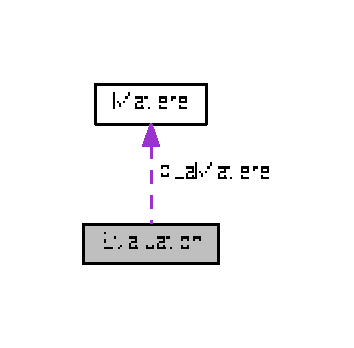
\includegraphics[width=170pt]{class_evaluation__coll__graph}
\end{center}
\end{figure}
\subsection*{Attributs privés}
\begin{DoxyCompactItemize}
\item 
string \hyperlink{class_evaluation_aaa4db227004bf8c359d863f6e1dbbefd}{evaluation\+Nom}
\item 
string \hyperlink{class_evaluation_ab9db02e7354335d10cf64c0b6d1e730f}{evaluation\+Date}
\item 
int \hyperlink{class_evaluation_ae000ec143562ed56975018bf82b13b5c}{semestre}
\item 
vector$<$ \hyperlink{class_note}{Note} $\ast$ $>$ \hyperlink{class_evaluation_ab235409526456cca10772832104f85f1}{vect\+Note}
\item 
\hyperlink{class_matiere}{Matiere} $\ast$ \hyperlink{class_evaluation_ad5f4d301c80076389e2ea31dfd7f09b1}{p\+La\+Matiere}
\end{DoxyCompactItemize}


\subsection{Description détaillée}
permet de creer des controles dans chaque matiere pour une section precise 

evaluation 

\subsection{Documentation des données membres}
\hypertarget{class_evaluation_ab9db02e7354335d10cf64c0b6d1e730f}{\index{Evaluation@{Evaluation}!evaluation\+Date@{evaluation\+Date}}
\index{evaluation\+Date@{evaluation\+Date}!Evaluation@{Evaluation}}
\subsubsection[{evaluation\+Date}]{\setlength{\rightskip}{0pt plus 5cm}string Evaluation\+::evaluation\+Date\hspace{0.3cm}{\ttfamily [private]}}}\label{class_evaluation_ab9db02e7354335d10cf64c0b6d1e730f}
\hypertarget{class_evaluation_aaa4db227004bf8c359d863f6e1dbbefd}{\index{Evaluation@{Evaluation}!evaluation\+Nom@{evaluation\+Nom}}
\index{evaluation\+Nom@{evaluation\+Nom}!Evaluation@{Evaluation}}
\subsubsection[{evaluation\+Nom}]{\setlength{\rightskip}{0pt plus 5cm}string Evaluation\+::evaluation\+Nom\hspace{0.3cm}{\ttfamily [private]}}}\label{class_evaluation_aaa4db227004bf8c359d863f6e1dbbefd}
\hypertarget{class_evaluation_ad5f4d301c80076389e2ea31dfd7f09b1}{\index{Evaluation@{Evaluation}!p\+La\+Matiere@{p\+La\+Matiere}}
\index{p\+La\+Matiere@{p\+La\+Matiere}!Evaluation@{Evaluation}}
\subsubsection[{p\+La\+Matiere}]{\setlength{\rightskip}{0pt plus 5cm}{\bf Matiere}$\ast$ Evaluation\+::p\+La\+Matiere\hspace{0.3cm}{\ttfamily [private]}}}\label{class_evaluation_ad5f4d301c80076389e2ea31dfd7f09b1}
\hypertarget{class_evaluation_ae000ec143562ed56975018bf82b13b5c}{\index{Evaluation@{Evaluation}!semestre@{semestre}}
\index{semestre@{semestre}!Evaluation@{Evaluation}}
\subsubsection[{semestre}]{\setlength{\rightskip}{0pt plus 5cm}int Evaluation\+::semestre\hspace{0.3cm}{\ttfamily [private]}}}\label{class_evaluation_ae000ec143562ed56975018bf82b13b5c}
\hypertarget{class_evaluation_ab235409526456cca10772832104f85f1}{\index{Evaluation@{Evaluation}!vect\+Note@{vect\+Note}}
\index{vect\+Note@{vect\+Note}!Evaluation@{Evaluation}}
\subsubsection[{vect\+Note}]{\setlength{\rightskip}{0pt plus 5cm}vector$<${\bf Note}$\ast$$>$ Evaluation\+::vect\+Note\hspace{0.3cm}{\ttfamily [private]}}}\label{class_evaluation_ab235409526456cca10772832104f85f1}


La documentation de cette classe a été générée à partir du fichier suivant \+:\begin{DoxyCompactItemize}
\item 
\hyperlink{evaluation_8h}{evaluation.\+h}\end{DoxyCompactItemize}

\hypertarget{class_matiere}{\section{Référence de la classe Matiere}
\label{class_matiere}\index{Matiere@{Matiere}}
}


{\ttfamily \#include $<$matiere.\+h$>$}

\subsection*{Fonctions membres publiques}
\begin{DoxyCompactItemize}
\item 
\hyperlink{class_matiere_a3776c9e9ec55c0073176ad3420fe7f52}{Matiere} (string \hyperlink{class_matiere_af3162fc28a37fac417cf01a3461f6265}{matiere\+Nom})
\item 
void \hyperlink{class_matiere_ab633e1c26288624667525b10af12d251}{afficher} ()
\item 
void \hyperlink{class_matiere_a516c86849342873a7148fe5668cbc7b1}{retour\+Application} ()
\item 
string \hyperlink{class_matiere_a722d95ed289dfca9ae90cbece33116de}{get\+Matiere\+Nom} ()
\item 
void \hyperlink{class_matiere_a558342de099d7fc21f5a37276fa6fae1}{afficher\+Matiere} ()
\end{DoxyCompactItemize}
\subsection*{Fonctions membres privées}
\begin{DoxyCompactItemize}
\item 
void \hyperlink{class_matiere_a97030f8ce6549e42648f1139e9641837}{ajouter\+Matiere} ()
\end{DoxyCompactItemize}
\subsection*{Attributs privés}
\begin{DoxyCompactItemize}
\item 
string \hyperlink{class_matiere_af3162fc28a37fac417cf01a3461f6265}{matiere\+Nom}
\end{DoxyCompactItemize}


\subsection{Documentation des constructeurs et destructeur}
\hypertarget{class_matiere_a3776c9e9ec55c0073176ad3420fe7f52}{\index{Matiere@{Matiere}!Matiere@{Matiere}}
\index{Matiere@{Matiere}!Matiere@{Matiere}}
\subsubsection[{Matiere}]{\setlength{\rightskip}{0pt plus 5cm}Matiere\+::\+Matiere (
\begin{DoxyParamCaption}
\item[{string}]{matiere\+Nom}
\end{DoxyParamCaption}
)}}\label{class_matiere_a3776c9e9ec55c0073176ad3420fe7f52}


\subsection{Documentation des fonctions membres}
\hypertarget{class_matiere_ab633e1c26288624667525b10af12d251}{\index{Matiere@{Matiere}!afficher@{afficher}}
\index{afficher@{afficher}!Matiere@{Matiere}}
\subsubsection[{afficher}]{\setlength{\rightskip}{0pt plus 5cm}void Matiere\+::afficher (
\begin{DoxyParamCaption}
{}
\end{DoxyParamCaption}
)}}\label{class_matiere_ab633e1c26288624667525b10af12d251}
\hypertarget{class_matiere_a558342de099d7fc21f5a37276fa6fae1}{\index{Matiere@{Matiere}!afficher\+Matiere@{afficher\+Matiere}}
\index{afficher\+Matiere@{afficher\+Matiere}!Matiere@{Matiere}}
\subsubsection[{afficher\+Matiere}]{\setlength{\rightskip}{0pt plus 5cm}void Matiere\+::afficher\+Matiere (
\begin{DoxyParamCaption}
{}
\end{DoxyParamCaption}
)}}\label{class_matiere_a558342de099d7fc21f5a37276fa6fae1}
\hypertarget{class_matiere_a97030f8ce6549e42648f1139e9641837}{\index{Matiere@{Matiere}!ajouter\+Matiere@{ajouter\+Matiere}}
\index{ajouter\+Matiere@{ajouter\+Matiere}!Matiere@{Matiere}}
\subsubsection[{ajouter\+Matiere}]{\setlength{\rightskip}{0pt plus 5cm}void Matiere\+::ajouter\+Matiere (
\begin{DoxyParamCaption}
{}
\end{DoxyParamCaption}
)\hspace{0.3cm}{\ttfamily [private]}}}\label{class_matiere_a97030f8ce6549e42648f1139e9641837}
\hypertarget{class_matiere_a722d95ed289dfca9ae90cbece33116de}{\index{Matiere@{Matiere}!get\+Matiere\+Nom@{get\+Matiere\+Nom}}
\index{get\+Matiere\+Nom@{get\+Matiere\+Nom}!Matiere@{Matiere}}
\subsubsection[{get\+Matiere\+Nom}]{\setlength{\rightskip}{0pt plus 5cm}string Matiere\+::get\+Matiere\+Nom (
\begin{DoxyParamCaption}
{}
\end{DoxyParamCaption}
)}}\label{class_matiere_a722d95ed289dfca9ae90cbece33116de}
\hypertarget{class_matiere_a516c86849342873a7148fe5668cbc7b1}{\index{Matiere@{Matiere}!retour\+Application@{retour\+Application}}
\index{retour\+Application@{retour\+Application}!Matiere@{Matiere}}
\subsubsection[{retour\+Application}]{\setlength{\rightskip}{0pt plus 5cm}void Matiere\+::retour\+Application (
\begin{DoxyParamCaption}
{}
\end{DoxyParamCaption}
)}}\label{class_matiere_a516c86849342873a7148fe5668cbc7b1}


\subsection{Documentation des données membres}
\hypertarget{class_matiere_af3162fc28a37fac417cf01a3461f6265}{\index{Matiere@{Matiere}!matiere\+Nom@{matiere\+Nom}}
\index{matiere\+Nom@{matiere\+Nom}!Matiere@{Matiere}}
\subsubsection[{matiere\+Nom}]{\setlength{\rightskip}{0pt plus 5cm}string Matiere\+::matiere\+Nom\hspace{0.3cm}{\ttfamily [private]}}}\label{class_matiere_af3162fc28a37fac417cf01a3461f6265}


La documentation de cette classe a été générée à partir des fichiers suivants \+:\begin{DoxyCompactItemize}
\item 
\hyperlink{matiere_8h}{matiere.\+h}\item 
\hyperlink{matiere_8cpp}{matiere.\+cpp}\end{DoxyCompactItemize}

\hypertarget{class_note}{\section{Référence de la classe Note}
\label{class_note}\index{Note@{Note}}
}


{\ttfamily \#include $<$note.\+h$>$}



Graphe de collaboration de Note\+:\nopagebreak
\begin{figure}[H]
\begin{center}
\leavevmode
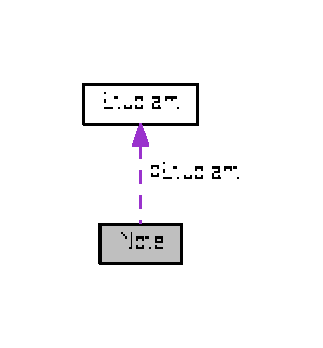
\includegraphics[width=155pt]{class_note__coll__graph}
\end{center}
\end{figure}
\subsection*{Attributs privés}
\begin{DoxyCompactItemize}
\item 
int \hyperlink{class_note_a3cb5f22dd5374f4e3c59c5f11dc7fbfb}{note}
\item 
vector$<$ int $>$ \hyperlink{class_note_a1e3b69349068565dc35fcae867145892}{vect\+Les\+Notes}
\item 
\hyperlink{class_etudiant}{Etudiant} $\ast$ \hyperlink{class_note_a3ceec90c97d49215fe0eaa33e92a83d2}{p\+Etudiant}
\end{DoxyCompactItemize}


\subsection{Documentation des données membres}
\hypertarget{class_note_a3cb5f22dd5374f4e3c59c5f11dc7fbfb}{\index{Note@{Note}!note@{note}}
\index{note@{note}!Note@{Note}}
\subsubsection[{note}]{\setlength{\rightskip}{0pt plus 5cm}int Note\+::note\hspace{0.3cm}{\ttfamily [private]}}}\label{class_note_a3cb5f22dd5374f4e3c59c5f11dc7fbfb}
\hypertarget{class_note_a3ceec90c97d49215fe0eaa33e92a83d2}{\index{Note@{Note}!p\+Etudiant@{p\+Etudiant}}
\index{p\+Etudiant@{p\+Etudiant}!Note@{Note}}
\subsubsection[{p\+Etudiant}]{\setlength{\rightskip}{0pt plus 5cm}{\bf Etudiant}$\ast$ Note\+::p\+Etudiant\hspace{0.3cm}{\ttfamily [private]}}}\label{class_note_a3ceec90c97d49215fe0eaa33e92a83d2}
\hypertarget{class_note_a1e3b69349068565dc35fcae867145892}{\index{Note@{Note}!vect\+Les\+Notes@{vect\+Les\+Notes}}
\index{vect\+Les\+Notes@{vect\+Les\+Notes}!Note@{Note}}
\subsubsection[{vect\+Les\+Notes}]{\setlength{\rightskip}{0pt plus 5cm}vector$<$int$>$ Note\+::vect\+Les\+Notes\hspace{0.3cm}{\ttfamily [private]}}}\label{class_note_a1e3b69349068565dc35fcae867145892}


La documentation de cette classe a été générée à partir du fichier suivant \+:\begin{DoxyCompactItemize}
\item 
\hyperlink{note_8h}{note.\+h}\end{DoxyCompactItemize}

\hypertarget{class_section}{\section{Référence de la classe Section}
\label{class_section}\index{Section@{Section}}
}


{\ttfamily \#include $<$section.\+h$>$}



Graphe de collaboration de Section\+:\nopagebreak
\begin{figure}[H]
\begin{center}
\leavevmode
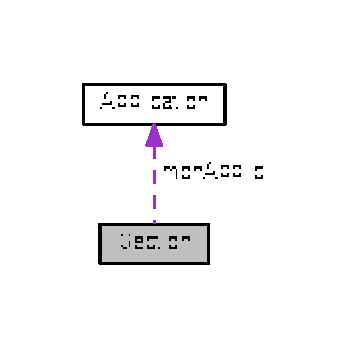
\includegraphics[width=166pt]{class_section__coll__graph}
\end{center}
\end{figure}
\subsection*{Fonctions membres publiques}
\begin{DoxyCompactItemize}
\item 
\hyperlink{class_section_abce12f33b3d02ae26aa071ee084379fb}{Section} (string \hyperlink{class_section_a4bb51bd5ac41f66e9935f8e1e46e1c45}{section\+Nom}, \hyperlink{class_application}{Application} $\ast$)
\begin{DoxyCompactList}\small\item\em constructeur de section creer un constructeur avec le nom de la section \end{DoxyCompactList}\item 
void \hyperlink{class_section_ad8bb64a516f00af11ec88262133936ff}{afficher\+Section} ()
\begin{DoxyCompactList}\small\item\em affichage section \end{DoxyCompactList}\item 
void \hyperlink{class_section_af9bc407774a67c0ce65d831fcf2005b2}{retour\+Application} ()
\begin{DoxyCompactList}\small\item\em retour \end{DoxyCompactList}\item 
string \hyperlink{class_section_a00b708087544f4830f3d8e115753e028}{get\+Section\+Nom} ()
\begin{DoxyCompactList}\small\item\em accesseur de section nom \end{DoxyCompactList}\item 
void \hyperlink{class_section_ad60532fac7868faad0b9b6ae413c860d}{run} ()
\begin{DoxyCompactList}\small\item\em execution \end{DoxyCompactList}\end{DoxyCompactItemize}
\subsection*{Fonctions membres privées}
\begin{DoxyCompactItemize}
\item 
void \hyperlink{class_section_a648fe297e7ba1d421517edfd50114bba}{affichage\+Du\+Choix\+Du\+Menu\+Secondaire} ()
\begin{DoxyCompactList}\small\item\em affichage du menu \end{DoxyCompactList}\item 
char \hyperlink{class_section_a1cfe7f586b0aa72fbdb4c66e3e760328}{saisie\+Controlee\+Du\+Choix\+Utilisateur\+Secondaire} ()
\begin{DoxyCompactList}\small\item\em controle saisie du choix \end{DoxyCompactList}\item 
void \hyperlink{class_section_a18d873239d981624af69451f4e804543}{choix\+Menu\+Application\+Secondaire} (char choix\+Util)
\begin{DoxyCompactList}\small\item\em choix utilisateur \end{DoxyCompactList}\item 
void \hyperlink{class_section_aca817449026803dfddfe01fb76b2a4d6}{ajouter\+Etudiant} ()
\begin{DoxyCompactList}\small\item\em creation etudiant \end{DoxyCompactList}\item 
void \hyperlink{class_section_a762dcfde40a8821f21324d1ade96999b}{afficher\+Etudiant} ()
\begin{DoxyCompactList}\small\item\em afficher etudiant \end{DoxyCompactList}\item 
void \hyperlink{class_section_a1c211fc04d2670f4d06623b3484e1456}{affecter\+Une\+Matiere} ()
\begin{DoxyCompactList}\small\item\em affectation d'une matiere \end{DoxyCompactList}\item 
void \hyperlink{class_section_a1debe78679287f470ce2ae2f8c5fd26d}{afficher\+Matiere} ()
\begin{DoxyCompactList}\small\item\em affichage matiere section \end{DoxyCompactList}\item 
void \hyperlink{class_section_a5947f98d44574643e111cc83c18a55c4}{ajouter\+Une\+Evaluation} ()
\begin{DoxyCompactList}\small\item\em creer une evaluation \end{DoxyCompactList}\item 
void \hyperlink{class_section_a7fa8e1804fc1643184330429cebc45af}{afficher\+Une\+Evaluation} ()
\begin{DoxyCompactList}\small\item\em afficher les evaluations \end{DoxyCompactList}\item 
void \hyperlink{class_section_abfb639b9563b4f0b00f9f8cdc6e28e65}{creer\+Tous\+Les\+Bulletins} ()
\begin{DoxyCompactList}\small\item\em creation bulletin \end{DoxyCompactList}\end{DoxyCompactItemize}
\subsection*{Attributs privés}
\begin{DoxyCompactItemize}
\item 
vector$<$ \hyperlink{class_matiere}{Matiere} $\ast$ $>$ \hyperlink{class_section_ac7febeae3b093a5cac9e9df3a7474fe4}{vect\+Les\+Matieres}
\begin{DoxyCompactList}\small\item\em vecteur matiere \end{DoxyCompactList}\item 
vector$<$ int $>$ \hyperlink{class_section_a189240ee9f2d58c63be99a7c65e9ec4f}{vect\+Les\+Coeff}
\begin{DoxyCompactList}\small\item\em coeff \end{DoxyCompactList}\item 
string \hyperlink{class_section_a4bb51bd5ac41f66e9935f8e1e46e1c45}{section\+Nom}
\begin{DoxyCompactList}\small\item\em nom de la section \end{DoxyCompactList}\item 
\hyperlink{class_application}{Application} $\ast$ \hyperlink{class_section_a387b69bedffb009e38d88cb272030bd4}{mon\+Applic}
\begin{DoxyCompactList}\small\item\em pointeur de l'application \end{DoxyCompactList}\item 
vector$<$ \hyperlink{class_evaluation}{Evaluation} $>$ \hyperlink{class_section_a2c07b1c98085111f120142cbe087fd36}{vect\+Evaluation}
\begin{DoxyCompactList}\small\item\em vecteur evaluation permet de recupere les differentes evaluations qui ont été faites \end{DoxyCompactList}\item 
vector$<$ \hyperlink{class_etudiant}{Etudiant} $>$ \hyperlink{class_section_a878e894d29cdbecf573949260a3be53e}{vect\+Etudiant}
\begin{DoxyCompactList}\small\item\em vecteur etudiant permet de recuperer les etudiants qui sont dans la sections \end{DoxyCompactList}\end{DoxyCompactItemize}


\subsection{Documentation des constructeurs et destructeur}
\hypertarget{class_section_abce12f33b3d02ae26aa071ee084379fb}{\index{Section@{Section}!Section@{Section}}
\index{Section@{Section}!Section@{Section}}
\subsubsection[{Section}]{\setlength{\rightskip}{0pt plus 5cm}Section\+::\+Section (
\begin{DoxyParamCaption}
\item[{string}]{section\+Nom, }
\item[{{\bf Application} $\ast$}]{l\+Applic}
\end{DoxyParamCaption}
)}}\label{class_section_abce12f33b3d02ae26aa071ee084379fb}


constructeur de section creer un constructeur avec le nom de la section 



\subsection{Documentation des fonctions membres}
\hypertarget{class_section_a1c211fc04d2670f4d06623b3484e1456}{\index{Section@{Section}!affecter\+Une\+Matiere@{affecter\+Une\+Matiere}}
\index{affecter\+Une\+Matiere@{affecter\+Une\+Matiere}!Section@{Section}}
\subsubsection[{affecter\+Une\+Matiere}]{\setlength{\rightskip}{0pt plus 5cm}void Section\+::affecter\+Une\+Matiere (
\begin{DoxyParamCaption}
{}
\end{DoxyParamCaption}
)\hspace{0.3cm}{\ttfamily [private]}}}\label{class_section_a1c211fc04d2670f4d06623b3484e1456}


affectation d'une matiere 

\begin{DoxyReturn}{Renvoie}
permet d'affecter les matieres que la section comporte 
\end{DoxyReturn}
\hypertarget{class_section_a648fe297e7ba1d421517edfd50114bba}{\index{Section@{Section}!affichage\+Du\+Choix\+Du\+Menu\+Secondaire@{affichage\+Du\+Choix\+Du\+Menu\+Secondaire}}
\index{affichage\+Du\+Choix\+Du\+Menu\+Secondaire@{affichage\+Du\+Choix\+Du\+Menu\+Secondaire}!Section@{Section}}
\subsubsection[{affichage\+Du\+Choix\+Du\+Menu\+Secondaire}]{\setlength{\rightskip}{0pt plus 5cm}void Section\+::affichage\+Du\+Choix\+Du\+Menu\+Secondaire (
\begin{DoxyParamCaption}
{}
\end{DoxyParamCaption}
)\hspace{0.3cm}{\ttfamily [private]}}}\label{class_section_a648fe297e7ba1d421517edfd50114bba}


affichage du menu 

\begin{DoxyReturn}{Renvoie}
affiche un menu de notre section avec les differentes possibilité 
\end{DoxyReturn}
\hypertarget{class_section_a762dcfde40a8821f21324d1ade96999b}{\index{Section@{Section}!afficher\+Etudiant@{afficher\+Etudiant}}
\index{afficher\+Etudiant@{afficher\+Etudiant}!Section@{Section}}
\subsubsection[{afficher\+Etudiant}]{\setlength{\rightskip}{0pt plus 5cm}void Section\+::afficher\+Etudiant (
\begin{DoxyParamCaption}
{}
\end{DoxyParamCaption}
)\hspace{0.3cm}{\ttfamily [private]}}}\label{class_section_a762dcfde40a8821f21324d1ade96999b}


afficher etudiant 

\begin{DoxyReturn}{Renvoie}
permet d'afficher la liste complete des etudiants de notre section 
\end{DoxyReturn}
\hypertarget{class_section_a1debe78679287f470ce2ae2f8c5fd26d}{\index{Section@{Section}!afficher\+Matiere@{afficher\+Matiere}}
\index{afficher\+Matiere@{afficher\+Matiere}!Section@{Section}}
\subsubsection[{afficher\+Matiere}]{\setlength{\rightskip}{0pt plus 5cm}void Section\+::afficher\+Matiere (
\begin{DoxyParamCaption}
{}
\end{DoxyParamCaption}
)\hspace{0.3cm}{\ttfamily [private]}}}\label{class_section_a1debe78679287f470ce2ae2f8c5fd26d}


affichage matiere section 

\begin{DoxyReturn}{Renvoie}
va affichger les matieres que la section comporte ainsi que le coefficient que la matiere comporte 
\end{DoxyReturn}
\hypertarget{class_section_ad8bb64a516f00af11ec88262133936ff}{\index{Section@{Section}!afficher\+Section@{afficher\+Section}}
\index{afficher\+Section@{afficher\+Section}!Section@{Section}}
\subsubsection[{afficher\+Section}]{\setlength{\rightskip}{0pt plus 5cm}void Section\+::afficher\+Section (
\begin{DoxyParamCaption}
{}
\end{DoxyParamCaption}
)}}\label{class_section_ad8bb64a516f00af11ec88262133936ff}


affichage section 

\begin{DoxyReturn}{Renvoie}
permet d'afficher les differentes sections que l'on dispose 
\end{DoxyReturn}
\hypertarget{class_section_a7fa8e1804fc1643184330429cebc45af}{\index{Section@{Section}!afficher\+Une\+Evaluation@{afficher\+Une\+Evaluation}}
\index{afficher\+Une\+Evaluation@{afficher\+Une\+Evaluation}!Section@{Section}}
\subsubsection[{afficher\+Une\+Evaluation}]{\setlength{\rightskip}{0pt plus 5cm}void Section\+::afficher\+Une\+Evaluation (
\begin{DoxyParamCaption}
{}
\end{DoxyParamCaption}
)\hspace{0.3cm}{\ttfamily [private]}}}\label{class_section_a7fa8e1804fc1643184330429cebc45af}


afficher les evaluations 

\begin{DoxyReturn}{Renvoie}
affichage des differentes evaluations que la section a eu ainsi que la moyenne de classe sur cette evaluations 
\end{DoxyReturn}
\hypertarget{class_section_aca817449026803dfddfe01fb76b2a4d6}{\index{Section@{Section}!ajouter\+Etudiant@{ajouter\+Etudiant}}
\index{ajouter\+Etudiant@{ajouter\+Etudiant}!Section@{Section}}
\subsubsection[{ajouter\+Etudiant}]{\setlength{\rightskip}{0pt plus 5cm}void Section\+::ajouter\+Etudiant (
\begin{DoxyParamCaption}
{}
\end{DoxyParamCaption}
)\hspace{0.3cm}{\ttfamily [private]}}}\label{class_section_aca817449026803dfddfe01fb76b2a4d6}


creation etudiant 

\begin{DoxyReturn}{Renvoie}
permet de rajouter un nouvelle etudiant a la section 
\end{DoxyReturn}
\hypertarget{class_section_a5947f98d44574643e111cc83c18a55c4}{\index{Section@{Section}!ajouter\+Une\+Evaluation@{ajouter\+Une\+Evaluation}}
\index{ajouter\+Une\+Evaluation@{ajouter\+Une\+Evaluation}!Section@{Section}}
\subsubsection[{ajouter\+Une\+Evaluation}]{\setlength{\rightskip}{0pt plus 5cm}void Section\+::ajouter\+Une\+Evaluation (
\begin{DoxyParamCaption}
{}
\end{DoxyParamCaption}
)\hspace{0.3cm}{\ttfamily [private]}}}\label{class_section_a5947f98d44574643e111cc83c18a55c4}


creer une evaluation 

\begin{DoxyReturn}{Renvoie}
permet de creer une evaluataion dans une matiere precise pour tous les eleves de la section 
\end{DoxyReturn}
\hypertarget{class_section_a18d873239d981624af69451f4e804543}{\index{Section@{Section}!choix\+Menu\+Application\+Secondaire@{choix\+Menu\+Application\+Secondaire}}
\index{choix\+Menu\+Application\+Secondaire@{choix\+Menu\+Application\+Secondaire}!Section@{Section}}
\subsubsection[{choix\+Menu\+Application\+Secondaire}]{\setlength{\rightskip}{0pt plus 5cm}void Section\+::choix\+Menu\+Application\+Secondaire (
\begin{DoxyParamCaption}
\item[{char}]{choix\+Util}
\end{DoxyParamCaption}
)\hspace{0.3cm}{\ttfamily [private]}}}\label{class_section_a18d873239d981624af69451f4e804543}


choix utilisateur 

\begin{DoxyReturn}{Renvoie}
permet d'executer le choix que l'utilisateur a choisi 
\end{DoxyReturn}
\hypertarget{class_section_abfb639b9563b4f0b00f9f8cdc6e28e65}{\index{Section@{Section}!creer\+Tous\+Les\+Bulletins@{creer\+Tous\+Les\+Bulletins}}
\index{creer\+Tous\+Les\+Bulletins@{creer\+Tous\+Les\+Bulletins}!Section@{Section}}
\subsubsection[{creer\+Tous\+Les\+Bulletins}]{\setlength{\rightskip}{0pt plus 5cm}void Section\+::creer\+Tous\+Les\+Bulletins (
\begin{DoxyParamCaption}
{}
\end{DoxyParamCaption}
)\hspace{0.3cm}{\ttfamily [private]}}}\label{class_section_abfb639b9563b4f0b00f9f8cdc6e28e65}


creation bulletin 

\begin{DoxyReturn}{Renvoie}
permet de creer l'integralité des bulletins pour la section mettra les notes de l'etudiant en fonction des differents controle et du coeff de la matiere la saisie d'un commentaire par eleve et matiere devra etre effectué 
\end{DoxyReturn}
\hypertarget{class_section_a00b708087544f4830f3d8e115753e028}{\index{Section@{Section}!get\+Section\+Nom@{get\+Section\+Nom}}
\index{get\+Section\+Nom@{get\+Section\+Nom}!Section@{Section}}
\subsubsection[{get\+Section\+Nom}]{\setlength{\rightskip}{0pt plus 5cm}string Section\+::get\+Section\+Nom (
\begin{DoxyParamCaption}
{}
\end{DoxyParamCaption}
)}}\label{class_section_a00b708087544f4830f3d8e115753e028}


accesseur de section nom 

\hypertarget{class_section_af9bc407774a67c0ce65d831fcf2005b2}{\index{Section@{Section}!retour\+Application@{retour\+Application}}
\index{retour\+Application@{retour\+Application}!Section@{Section}}
\subsubsection[{retour\+Application}]{\setlength{\rightskip}{0pt plus 5cm}void Section\+::retour\+Application (
\begin{DoxyParamCaption}
{}
\end{DoxyParamCaption}
)}}\label{class_section_af9bc407774a67c0ce65d831fcf2005b2}


retour 

\begin{DoxyReturn}{Renvoie}
permet de retourner au pmenu de l'application 
\end{DoxyReturn}
\hypertarget{class_section_ad60532fac7868faad0b9b6ae413c860d}{\index{Section@{Section}!run@{run}}
\index{run@{run}!Section@{Section}}
\subsubsection[{run}]{\setlength{\rightskip}{0pt plus 5cm}void Section\+::run (
\begin{DoxyParamCaption}
{}
\end{DoxyParamCaption}
)}}\label{class_section_ad60532fac7868faad0b9b6ae413c860d}


execution 

\begin{DoxyReturn}{Renvoie}
permet d'executer le code de la section et quil se repete 
\end{DoxyReturn}
\hypertarget{class_section_a1cfe7f586b0aa72fbdb4c66e3e760328}{\index{Section@{Section}!saisie\+Controlee\+Du\+Choix\+Utilisateur\+Secondaire@{saisie\+Controlee\+Du\+Choix\+Utilisateur\+Secondaire}}
\index{saisie\+Controlee\+Du\+Choix\+Utilisateur\+Secondaire@{saisie\+Controlee\+Du\+Choix\+Utilisateur\+Secondaire}!Section@{Section}}
\subsubsection[{saisie\+Controlee\+Du\+Choix\+Utilisateur\+Secondaire}]{\setlength{\rightskip}{0pt plus 5cm}char Section\+::saisie\+Controlee\+Du\+Choix\+Utilisateur\+Secondaire (
\begin{DoxyParamCaption}
{}
\end{DoxyParamCaption}
)\hspace{0.3cm}{\ttfamily [private]}}}\label{class_section_a1cfe7f586b0aa72fbdb4c66e3e760328}


controle saisie du choix 

\begin{DoxyReturn}{Renvoie}
permet de verifier que notre utilisateur a taper un choix qui est valide evite les erreurs de frappe 
\end{DoxyReturn}


\subsection{Documentation des données membres}
\hypertarget{class_section_a387b69bedffb009e38d88cb272030bd4}{\index{Section@{Section}!mon\+Applic@{mon\+Applic}}
\index{mon\+Applic@{mon\+Applic}!Section@{Section}}
\subsubsection[{mon\+Applic}]{\setlength{\rightskip}{0pt plus 5cm}{\bf Application}$\ast$ Section\+::mon\+Applic\hspace{0.3cm}{\ttfamily [private]}}}\label{class_section_a387b69bedffb009e38d88cb272030bd4}


pointeur de l'application 

\begin{DoxyReturn}{Renvoie}
c'est un pointeur de la classe application qui porte le nom du nom de mon apllication 
\end{DoxyReturn}
\hypertarget{class_section_a4bb51bd5ac41f66e9935f8e1e46e1c45}{\index{Section@{Section}!section\+Nom@{section\+Nom}}
\index{section\+Nom@{section\+Nom}!Section@{Section}}
\subsubsection[{section\+Nom}]{\setlength{\rightskip}{0pt plus 5cm}string Section\+::section\+Nom\hspace{0.3cm}{\ttfamily [private]}}}\label{class_section_a4bb51bd5ac41f66e9935f8e1e46e1c45}


nom de la section 

\begin{DoxyReturn}{Renvoie}
permet d'avoir une variable contenant le nom de la section 
\end{DoxyReturn}
\hypertarget{class_section_a878e894d29cdbecf573949260a3be53e}{\index{Section@{Section}!vect\+Etudiant@{vect\+Etudiant}}
\index{vect\+Etudiant@{vect\+Etudiant}!Section@{Section}}
\subsubsection[{vect\+Etudiant}]{\setlength{\rightskip}{0pt plus 5cm}vector$<${\bf Etudiant}$>$ Section\+::vect\+Etudiant\hspace{0.3cm}{\ttfamily [private]}}}\label{class_section_a878e894d29cdbecf573949260a3be53e}


vecteur etudiant permet de recuperer les etudiants qui sont dans la sections 

\hypertarget{class_section_a2c07b1c98085111f120142cbe087fd36}{\index{Section@{Section}!vect\+Evaluation@{vect\+Evaluation}}
\index{vect\+Evaluation@{vect\+Evaluation}!Section@{Section}}
\subsubsection[{vect\+Evaluation}]{\setlength{\rightskip}{0pt plus 5cm}vector$<${\bf Evaluation}$>$ Section\+::vect\+Evaluation\hspace{0.3cm}{\ttfamily [private]}}}\label{class_section_a2c07b1c98085111f120142cbe087fd36}


vecteur evaluation permet de recupere les differentes evaluations qui ont été faites 

\hypertarget{class_section_a189240ee9f2d58c63be99a7c65e9ec4f}{\index{Section@{Section}!vect\+Les\+Coeff@{vect\+Les\+Coeff}}
\index{vect\+Les\+Coeff@{vect\+Les\+Coeff}!Section@{Section}}
\subsubsection[{vect\+Les\+Coeff}]{\setlength{\rightskip}{0pt plus 5cm}vector$<$int$>$ Section\+::vect\+Les\+Coeff\hspace{0.3cm}{\ttfamily [private]}}}\label{class_section_a189240ee9f2d58c63be99a7c65e9ec4f}


coeff 

\begin{DoxyReturn}{Renvoie}
permet d'affecter un coeeficient à une matiere et cela en focntion des sections 
\end{DoxyReturn}
\hypertarget{class_section_ac7febeae3b093a5cac9e9df3a7474fe4}{\index{Section@{Section}!vect\+Les\+Matieres@{vect\+Les\+Matieres}}
\index{vect\+Les\+Matieres@{vect\+Les\+Matieres}!Section@{Section}}
\subsubsection[{vect\+Les\+Matieres}]{\setlength{\rightskip}{0pt plus 5cm}vector$<${\bf Matiere}$\ast$$>$ Section\+::vect\+Les\+Matieres\hspace{0.3cm}{\ttfamily [private]}}}\label{class_section_ac7febeae3b093a5cac9e9df3a7474fe4}


vecteur matiere 

\begin{DoxyReturn}{Renvoie}
pour recuperer les matieres grace au pointeur 
\end{DoxyReturn}


La documentation de cette classe a été générée à partir des fichiers suivants \+:\begin{DoxyCompactItemize}
\item 
\hyperlink{section_8h}{section.\+h}\item 
\hyperlink{section_8cpp}{section.\+cpp}\end{DoxyCompactItemize}

\chapter{Documentation des fichiers}
\hypertarget{application_8cpp}{\section{Référence du fichier application.\+cpp}
\label{application_8cpp}\index{application.\+cpp@{application.\+cpp}}
}
{\ttfamily \#include \char`\"{}application.\+h\char`\"{}}\\*
{\ttfamily \#include $<$cstdlib$>$}\\*
Graphe des dépendances par inclusion de application.\+cpp\+:\nopagebreak
\begin{figure}[H]
\begin{center}
\leavevmode
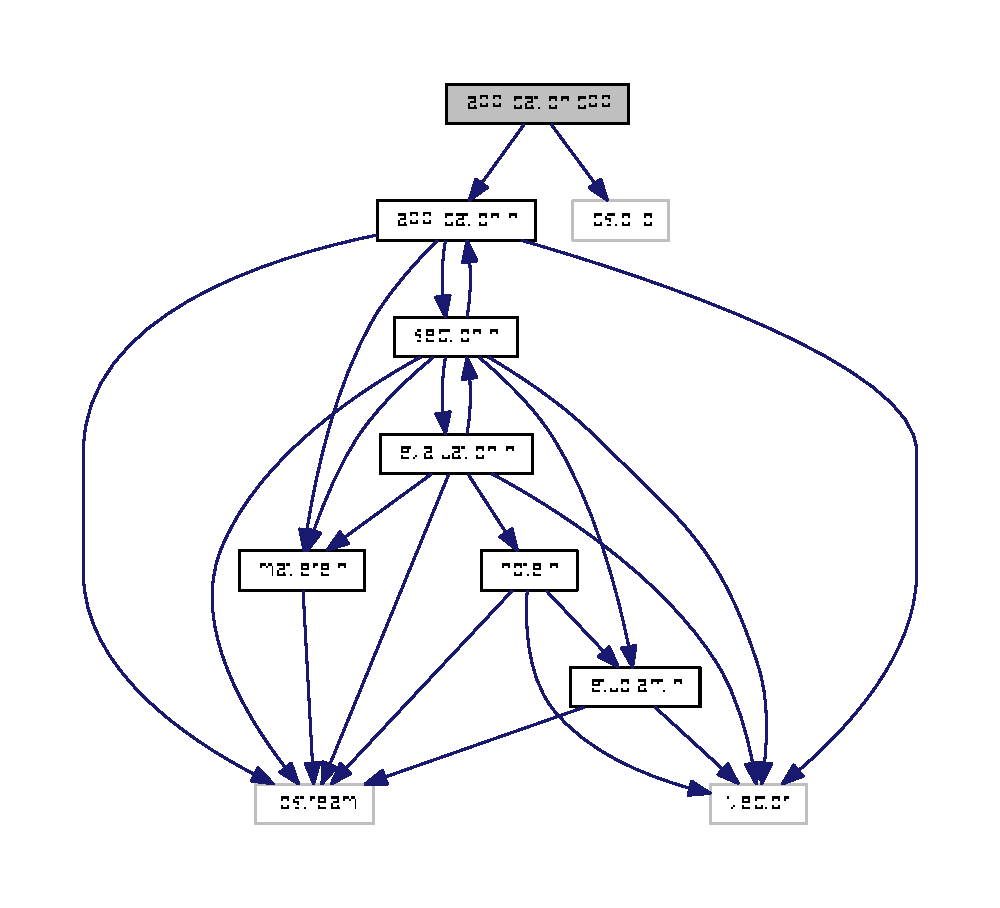
\includegraphics[width=350pt]{application_8cpp__incl}
\end{center}
\end{figure}

\hypertarget{application_8h}{\section{Référence du fichier application.\+h}
\label{application_8h}\index{application.\+h@{application.\+h}}
}
{\ttfamily \#include $<$iostream$>$}\\*
{\ttfamily \#include $<$vector$>$}\\*
{\ttfamily \#include \char`\"{}section.\+h\char`\"{}}\\*
{\ttfamily \#include \char`\"{}matiere.\+h\char`\"{}}\\*
Graphe des dépendances par inclusion de application.\+h\+:\nopagebreak
\begin{figure}[H]
\begin{center}
\leavevmode
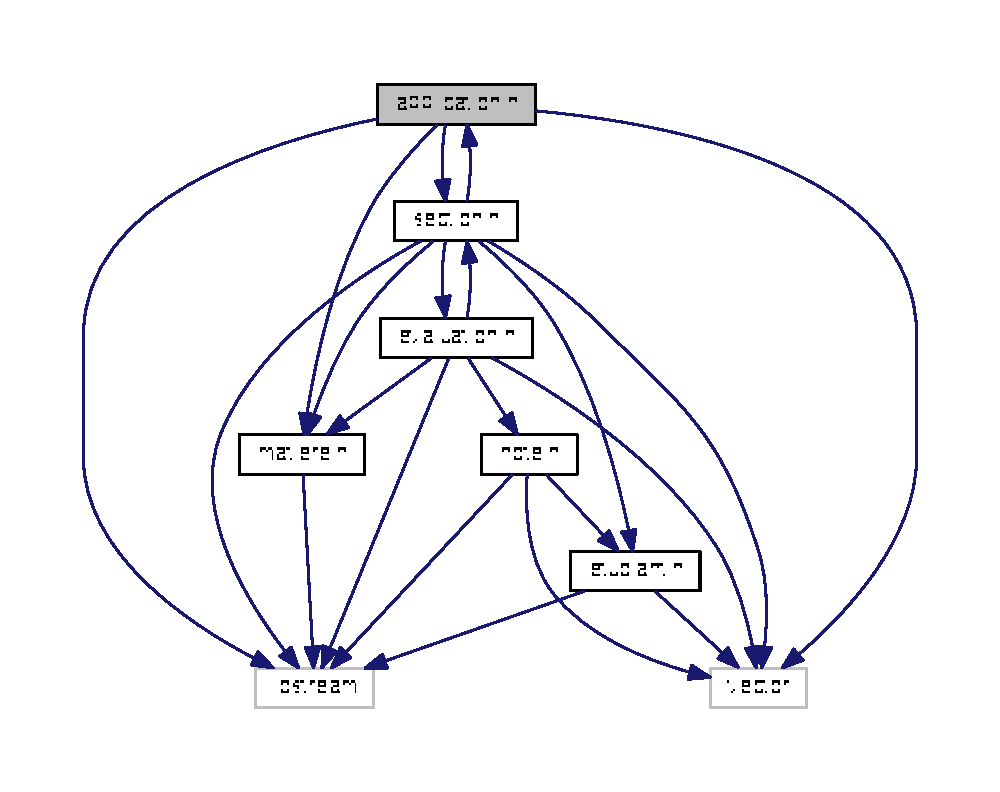
\includegraphics[width=350pt]{application_8h__incl}
\end{center}
\end{figure}
Ce graphe montre quels fichiers incluent directement ou indirectement ce fichier \+:\nopagebreak
\begin{figure}[H]
\begin{center}
\leavevmode
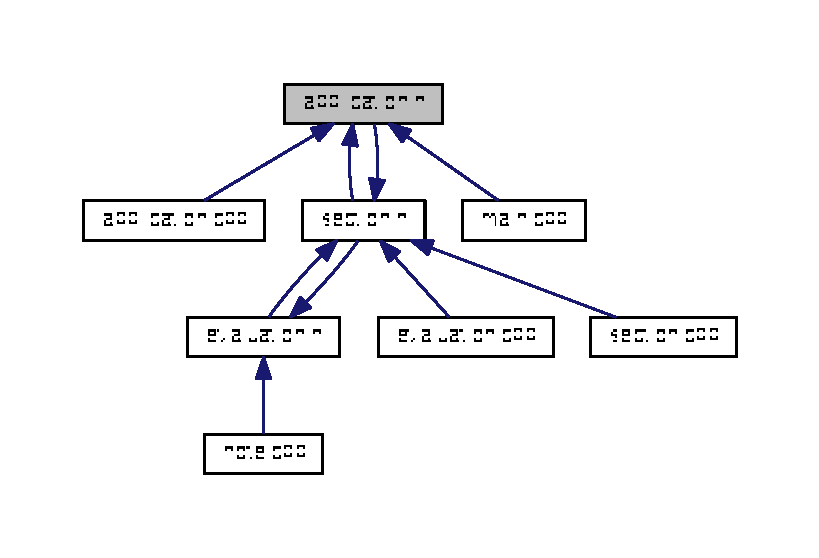
\includegraphics[width=350pt]{application_8h__dep__incl}
\end{center}
\end{figure}
\subsection*{Classes}
\begin{DoxyCompactItemize}
\item 
class \hyperlink{class_application}{Application}
\end{DoxyCompactItemize}

\hypertarget{bulletin_8cpp}{\section{Référence du fichier bulletin.\+cpp}
\label{bulletin_8cpp}\index{bulletin.\+cpp@{bulletin.\+cpp}}
}
{\ttfamily \#include \char`\"{}bulletin.\+h\char`\"{}}\\*
Graphe des dépendances par inclusion de bulletin.\+cpp\+:\nopagebreak
\begin{figure}[H]
\begin{center}
\leavevmode
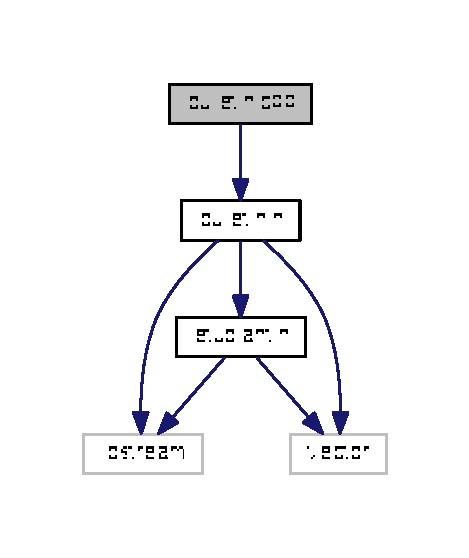
\includegraphics[width=225pt]{bulletin_8cpp__incl}
\end{center}
\end{figure}

\hypertarget{bulletin_8h}{\section{Référence du fichier bulletin.\+h}
\label{bulletin_8h}\index{bulletin.\+h@{bulletin.\+h}}
}
{\ttfamily \#include $<$iostream$>$}\\*
{\ttfamily \#include $<$vector$>$}\\*
{\ttfamily \#include \char`\"{}etudiant.\+h\char`\"{}}\\*
Graphe des dépendances par inclusion de bulletin.\+h\+:\nopagebreak
\begin{figure}[H]
\begin{center}
\leavevmode
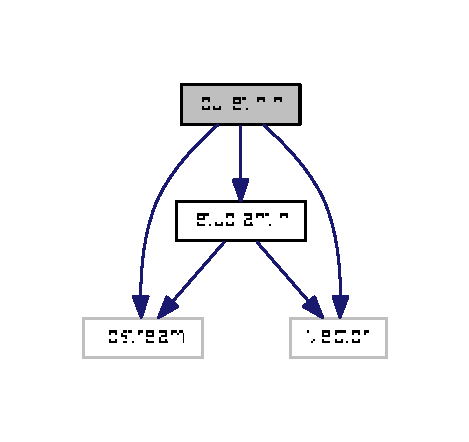
\includegraphics[width=225pt]{bulletin_8h__incl}
\end{center}
\end{figure}
Ce graphe montre quels fichiers incluent directement ou indirectement ce fichier \+:\nopagebreak
\begin{figure}[H]
\begin{center}
\leavevmode
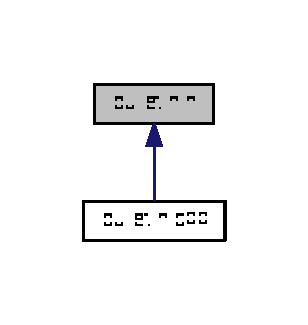
\includegraphics[width=148pt]{bulletin_8h__dep__incl}
\end{center}
\end{figure}
\subsection*{Classes}
\begin{DoxyCompactItemize}
\item 
class \hyperlink{class_bulletin}{Bulletin}
\end{DoxyCompactItemize}
\subsection*{Macros}
\begin{DoxyCompactItemize}
\item 
\#define \hyperlink{bulletin_8h_a796bd7c6ba2e59281760fb155c6287e8}{A\+P\+P\+L\+I\+C\+A\+T\+I\+O\+N}
\end{DoxyCompactItemize}


\subsection{Documentation des macros}
\hypertarget{bulletin_8h_a796bd7c6ba2e59281760fb155c6287e8}{\index{bulletin.\+h@{bulletin.\+h}!A\+P\+P\+L\+I\+C\+A\+T\+I\+O\+N@{A\+P\+P\+L\+I\+C\+A\+T\+I\+O\+N}}
\index{A\+P\+P\+L\+I\+C\+A\+T\+I\+O\+N@{A\+P\+P\+L\+I\+C\+A\+T\+I\+O\+N}!bulletin.\+h@{bulletin.\+h}}
\subsubsection[{A\+P\+P\+L\+I\+C\+A\+T\+I\+O\+N}]{\setlength{\rightskip}{0pt plus 5cm}\#define A\+P\+P\+L\+I\+C\+A\+T\+I\+O\+N}}\label{bulletin_8h_a796bd7c6ba2e59281760fb155c6287e8}

\hypertarget{etudiant_8cpp}{\section{Référence du fichier etudiant.\+cpp}
\label{etudiant_8cpp}\index{etudiant.\+cpp@{etudiant.\+cpp}}
}
{\ttfamily \#include \char`\"{}etudiant.\+h\char`\"{}}\\*
Graphe des dépendances par inclusion de etudiant.\+cpp\+:\nopagebreak
\begin{figure}[H]
\begin{center}
\leavevmode
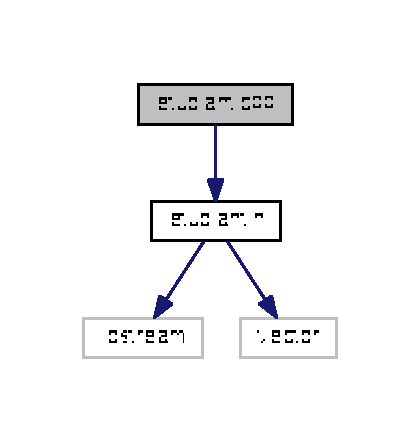
\includegraphics[width=201pt]{etudiant_8cpp__incl}
\end{center}
\end{figure}

\hypertarget{etudiant_8h}{\section{Référence du fichier etudiant.\+h}
\label{etudiant_8h}\index{etudiant.\+h@{etudiant.\+h}}
}
{\ttfamily \#include $<$iostream$>$}\\*
{\ttfamily \#include $<$vector$>$}\\*
Graphe des dépendances par inclusion de etudiant.\+h\+:\nopagebreak
\begin{figure}[H]
\begin{center}
\leavevmode
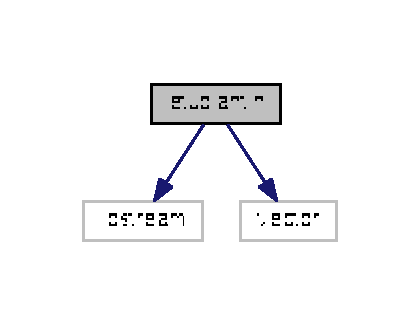
\includegraphics[width=201pt]{etudiant_8h__incl}
\end{center}
\end{figure}
Ce graphe montre quels fichiers incluent directement ou indirectement ce fichier \+:\nopagebreak
\begin{figure}[H]
\begin{center}
\leavevmode
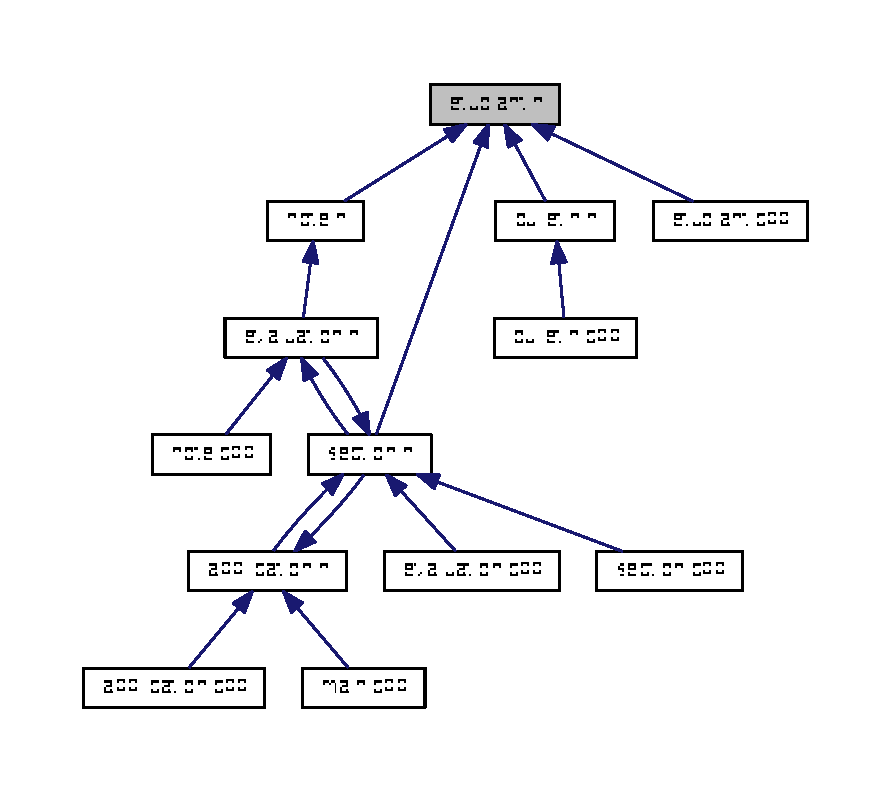
\includegraphics[width=350pt]{etudiant_8h__dep__incl}
\end{center}
\end{figure}
\subsection*{Classes}
\begin{DoxyCompactItemize}
\item 
class \hyperlink{class_etudiant}{Etudiant}
\end{DoxyCompactItemize}

\hypertarget{evaluation_8cpp}{\section{Référence du fichier evaluation.\+cpp}
\label{evaluation_8cpp}\index{evaluation.\+cpp@{evaluation.\+cpp}}
}
{\ttfamily \#include \char`\"{}section.\+h\char`\"{}}\\*
Graphe des dépendances par inclusion de evaluation.\+cpp\+:\nopagebreak
\begin{figure}[H]
\begin{center}
\leavevmode
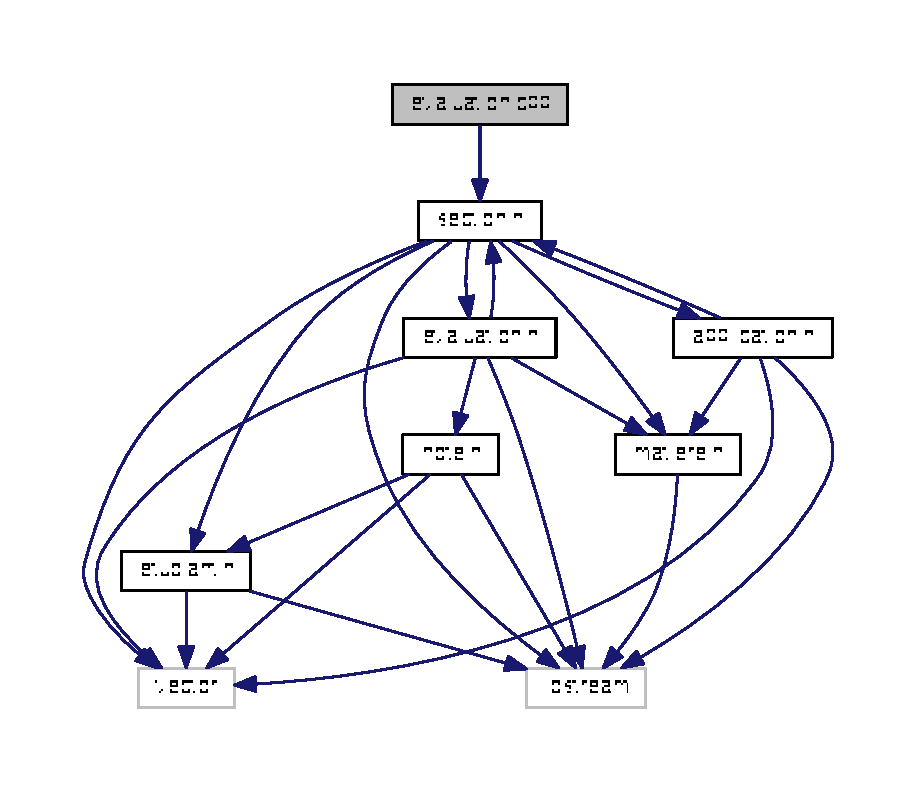
\includegraphics[width=350pt]{evaluation_8cpp__incl}
\end{center}
\end{figure}

\hypertarget{evaluation_8h}{\section{Référence du fichier evaluation.\+h}
\label{evaluation_8h}\index{evaluation.\+h@{evaluation.\+h}}
}
{\ttfamily \#include $<$iostream$>$}\\*
{\ttfamily \#include $<$vector$>$}\\*
{\ttfamily \#include \char`\"{}section.\+h\char`\"{}}\\*
{\ttfamily \#include \char`\"{}matiere.\+h\char`\"{}}\\*
{\ttfamily \#include \char`\"{}note.\+h\char`\"{}}\\*
Graphe des dépendances par inclusion de evaluation.\+h\+:\nopagebreak
\begin{figure}[H]
\begin{center}
\leavevmode
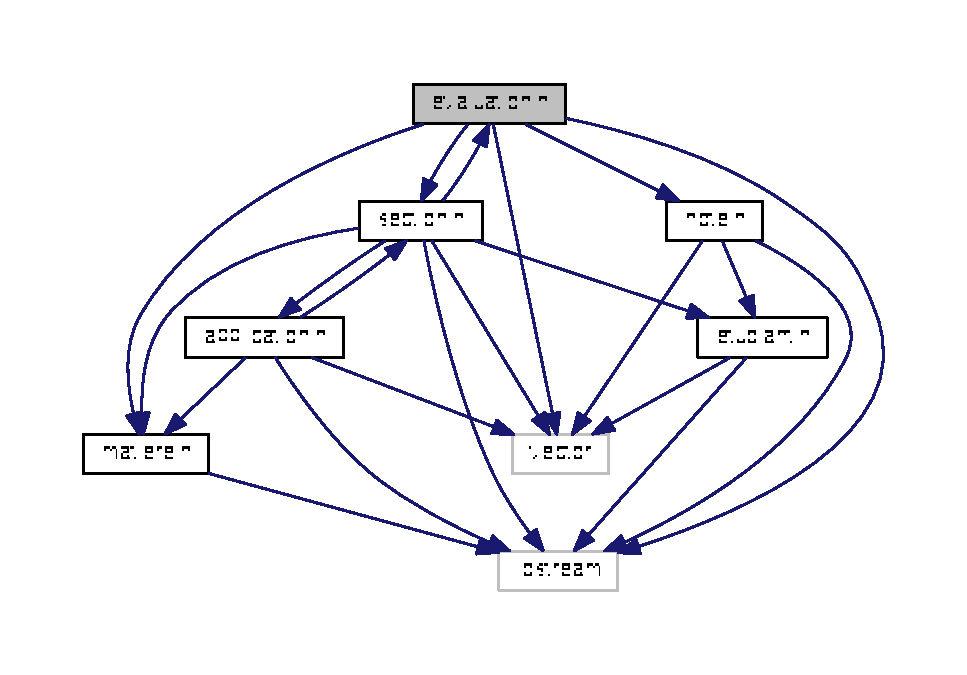
\includegraphics[width=350pt]{evaluation_8h__incl}
\end{center}
\end{figure}
Ce graphe montre quels fichiers incluent directement ou indirectement ce fichier \+:\nopagebreak
\begin{figure}[H]
\begin{center}
\leavevmode
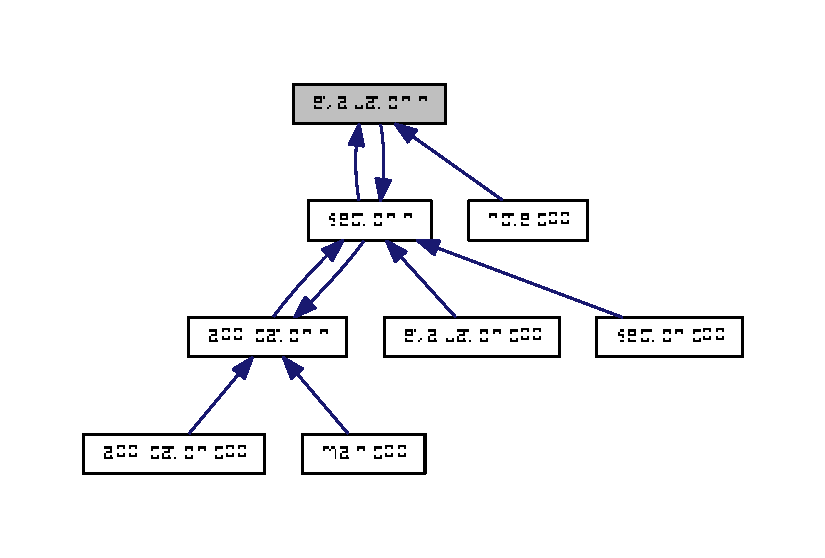
\includegraphics[width=350pt]{evaluation_8h__dep__incl}
\end{center}
\end{figure}
\subsection*{Classes}
\begin{DoxyCompactItemize}
\item 
class \hyperlink{class_evaluation}{Evaluation}
\begin{DoxyCompactList}\small\item\em permet de creer des controles dans chaque matiere pour une section precise \end{DoxyCompactList}\end{DoxyCompactItemize}

\hypertarget{main_8cpp}{\section{Référence du fichier main.\+cpp}
\label{main_8cpp}\index{main.\+cpp@{main.\+cpp}}
}
{\ttfamily \#include \char`\"{}application.\+h\char`\"{}}\\*
Graphe des dépendances par inclusion de main.\+cpp\+:\nopagebreak
\begin{figure}[H]
\begin{center}
\leavevmode
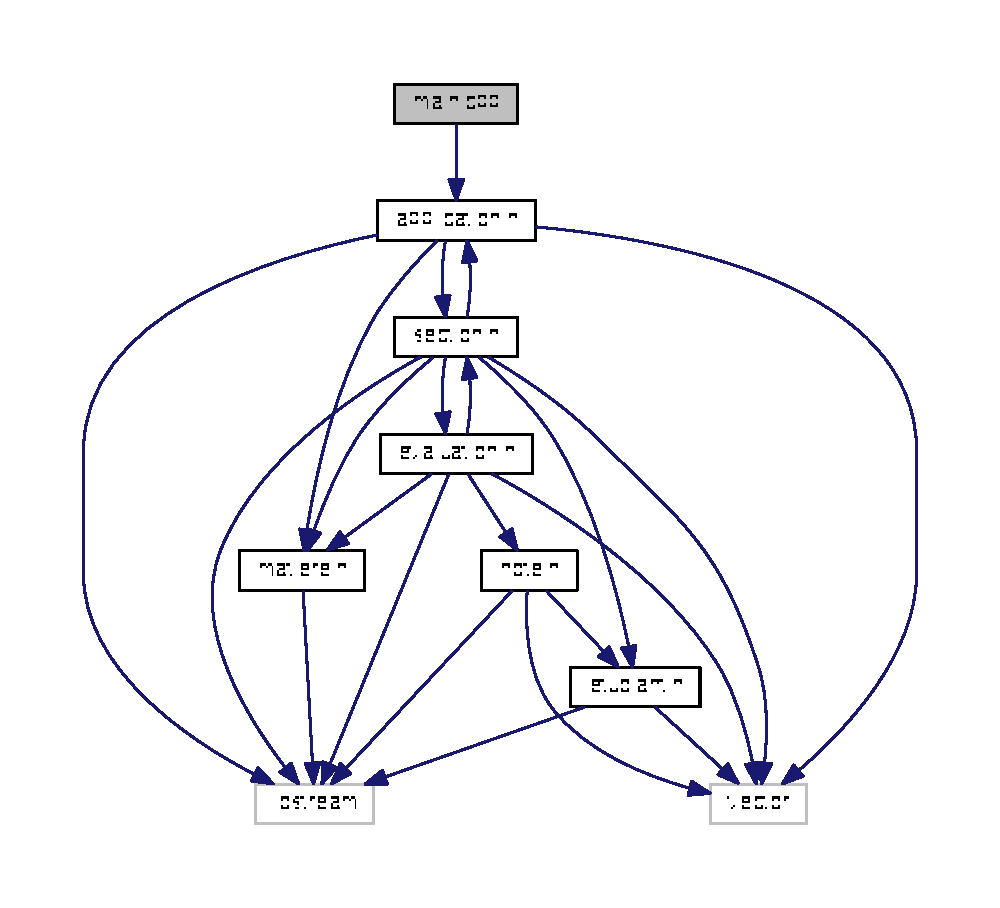
\includegraphics[width=350pt]{main_8cpp__incl}
\end{center}
\end{figure}
\subsection*{Fonctions}
\begin{DoxyCompactItemize}
\item 
int \hyperlink{main_8cpp_ae66f6b31b5ad750f1fe042a706a4e3d4}{main} ()
\end{DoxyCompactItemize}


\subsection{Documentation des fonctions}
\hypertarget{main_8cpp_ae66f6b31b5ad750f1fe042a706a4e3d4}{\index{main.\+cpp@{main.\+cpp}!main@{main}}
\index{main@{main}!main.\+cpp@{main.\+cpp}}
\subsubsection[{main}]{\setlength{\rightskip}{0pt plus 5cm}int main (
\begin{DoxyParamCaption}
{}
\end{DoxyParamCaption}
)}}\label{main_8cpp_ae66f6b31b5ad750f1fe042a706a4e3d4}

\hypertarget{matiere_8cpp}{\section{Référence du fichier matiere.\+cpp}
\label{matiere_8cpp}\index{matiere.\+cpp@{matiere.\+cpp}}
}
{\ttfamily \#include \char`\"{}matiere.\+h\char`\"{}}\\*
Graphe des dépendances par inclusion de matiere.\+cpp\+:\nopagebreak
\begin{figure}[H]
\begin{center}
\leavevmode
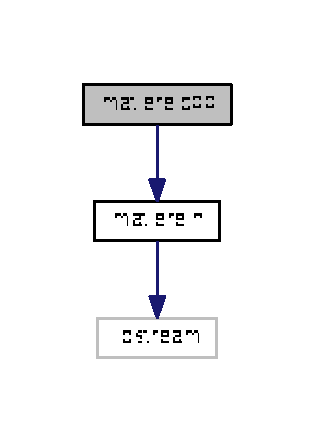
\includegraphics[width=151pt]{matiere_8cpp__incl}
\end{center}
\end{figure}

\hypertarget{matiere_8h}{\section{Référence du fichier matiere.\+h}
\label{matiere_8h}\index{matiere.\+h@{matiere.\+h}}
}
{\ttfamily \#include $<$iostream$>$}\\*
Graphe des dépendances par inclusion de matiere.\+h\+:\nopagebreak
\begin{figure}[H]
\begin{center}
\leavevmode
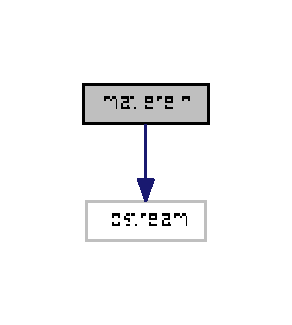
\includegraphics[width=140pt]{matiere_8h__incl}
\end{center}
\end{figure}
Ce graphe montre quels fichiers incluent directement ou indirectement ce fichier \+:\nopagebreak
\begin{figure}[H]
\begin{center}
\leavevmode
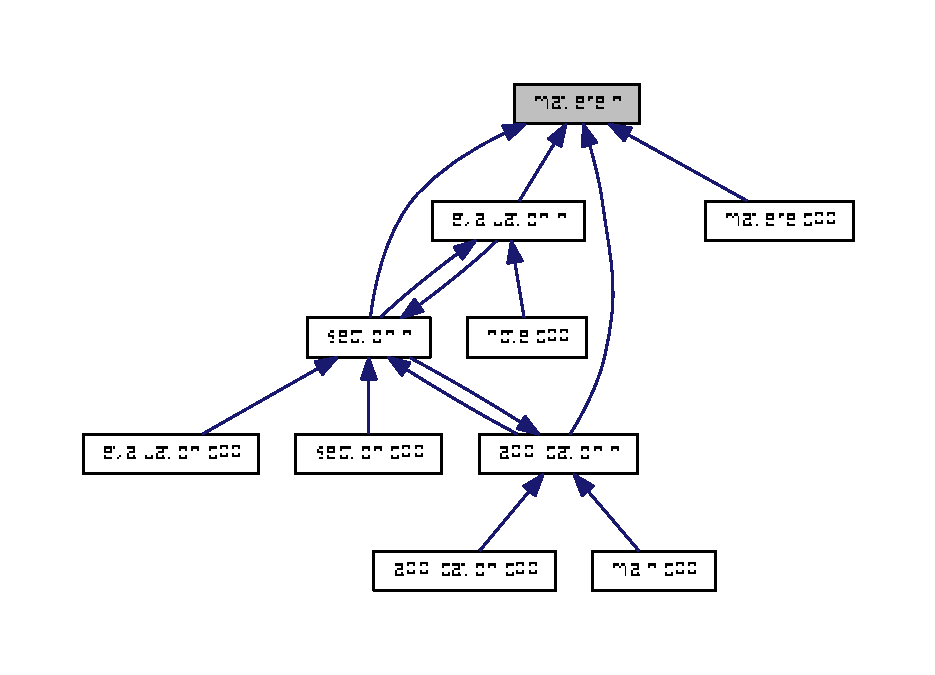
\includegraphics[width=350pt]{matiere_8h__dep__incl}
\end{center}
\end{figure}
\subsection*{Classes}
\begin{DoxyCompactItemize}
\item 
class \hyperlink{class_matiere}{Matiere}
\end{DoxyCompactItemize}

\hypertarget{note_8cpp}{\section{Référence du fichier note.\+cpp}
\label{note_8cpp}\index{note.\+cpp@{note.\+cpp}}
}
{\ttfamily \#include \char`\"{}evaluation.\+h\char`\"{}}\\*
Graphe des dépendances par inclusion de note.\+cpp\+:\nopagebreak
\begin{figure}[H]
\begin{center}
\leavevmode
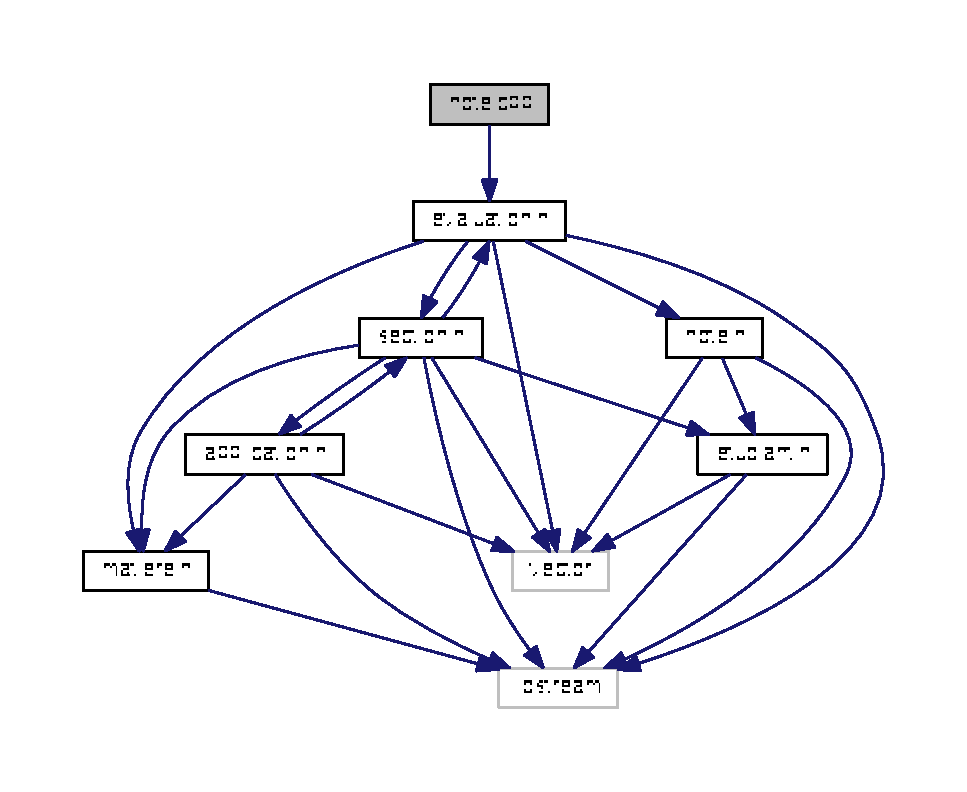
\includegraphics[width=350pt]{note_8cpp__incl}
\end{center}
\end{figure}

\hypertarget{note_8h}{\section{Référence du fichier note.\+h}
\label{note_8h}\index{note.\+h@{note.\+h}}
}
{\ttfamily \#include $<$iostream$>$}\\*
{\ttfamily \#include $<$vector$>$}\\*
{\ttfamily \#include \char`\"{}etudiant.\+h\char`\"{}}\\*
Graphe des dépendances par inclusion de note.\+h\+:\nopagebreak
\begin{figure}[H]
\begin{center}
\leavevmode
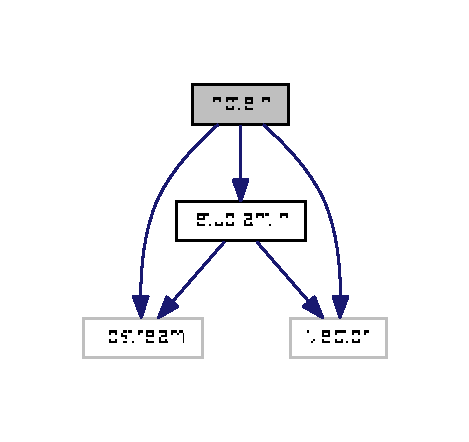
\includegraphics[width=225pt]{note_8h__incl}
\end{center}
\end{figure}
Ce graphe montre quels fichiers incluent directement ou indirectement ce fichier \+:\nopagebreak
\begin{figure}[H]
\begin{center}
\leavevmode
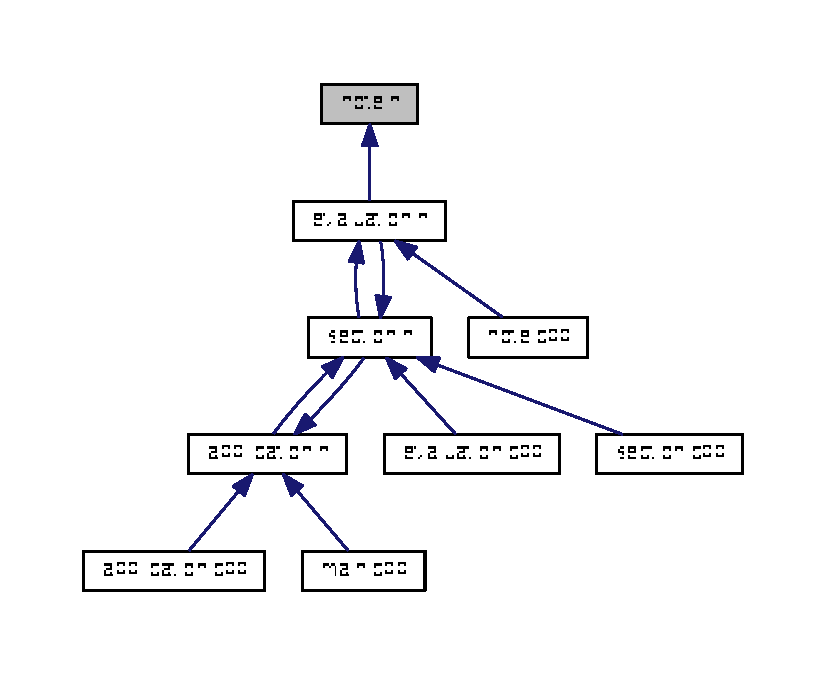
\includegraphics[width=350pt]{note_8h__dep__incl}
\end{center}
\end{figure}
\subsection*{Classes}
\begin{DoxyCompactItemize}
\item 
class \hyperlink{class_note}{Note}
\end{DoxyCompactItemize}

\hypertarget{section_8cpp}{\section{Référence du fichier section.\+cpp}
\label{section_8cpp}\index{section.\+cpp@{section.\+cpp}}
}
{\ttfamily \#include \char`\"{}section.\+h\char`\"{}}\\*
Graphe des dépendances par inclusion de section.\+cpp\+:\nopagebreak
\begin{figure}[H]
\begin{center}
\leavevmode
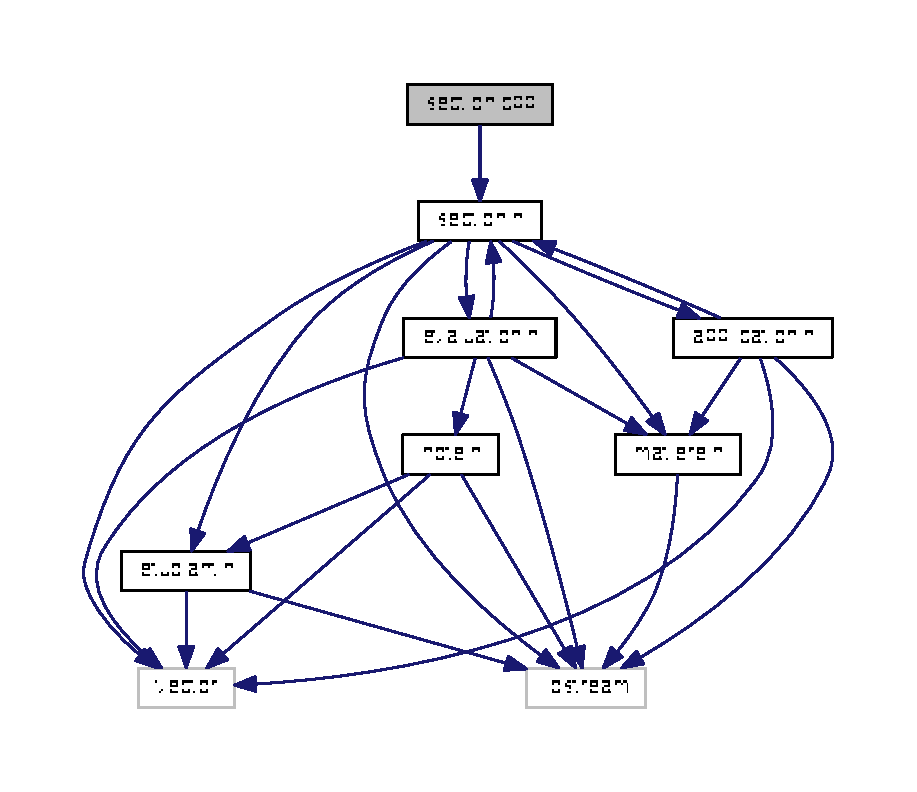
\includegraphics[width=350pt]{section_8cpp__incl}
\end{center}
\end{figure}

\hypertarget{section_8h}{\section{Référence du fichier section.\+h}
\label{section_8h}\index{section.\+h@{section.\+h}}
}
{\ttfamily \#include $<$iostream$>$}\\*
{\ttfamily \#include $<$vector$>$}\\*
{\ttfamily \#include \char`\"{}evaluation.\+h\char`\"{}}\\*
{\ttfamily \#include \char`\"{}etudiant.\+h\char`\"{}}\\*
{\ttfamily \#include \char`\"{}matiere.\+h\char`\"{}}\\*
{\ttfamily \#include \char`\"{}application.\+h\char`\"{}}\\*
Graphe des dépendances par inclusion de section.\+h\+:\nopagebreak
\begin{figure}[H]
\begin{center}
\leavevmode
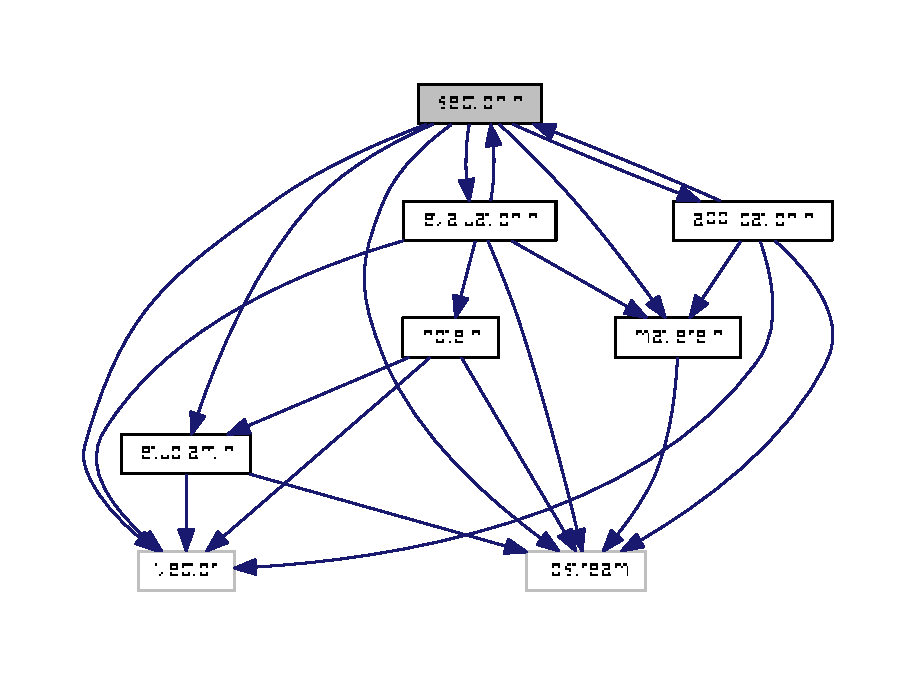
\includegraphics[width=350pt]{section_8h__incl}
\end{center}
\end{figure}
Ce graphe montre quels fichiers incluent directement ou indirectement ce fichier \+:\nopagebreak
\begin{figure}[H]
\begin{center}
\leavevmode
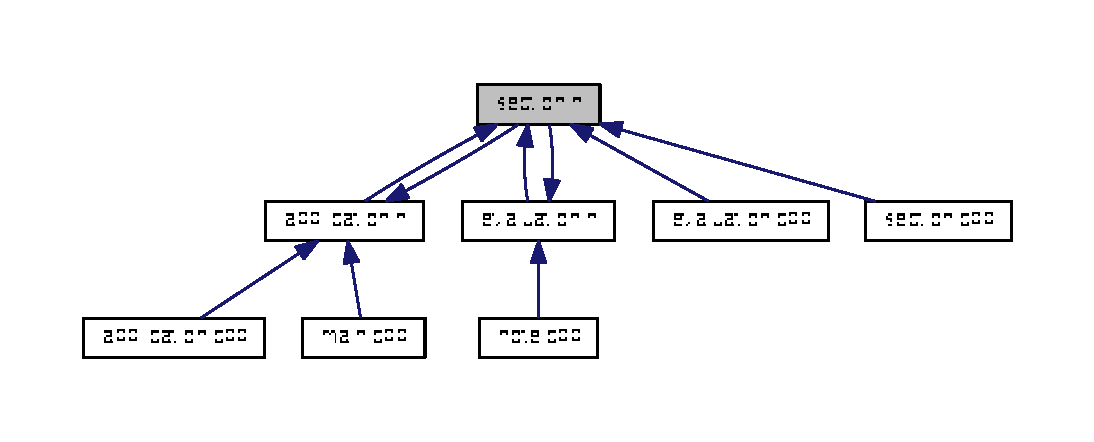
\includegraphics[width=350pt]{section_8h__dep__incl}
\end{center}
\end{figure}
\subsection*{Classes}
\begin{DoxyCompactItemize}
\item 
class \hyperlink{class_section}{Section}
\end{DoxyCompactItemize}

%--- End generated contents ---

% Index
\newpage
\phantomsection
\addcontentsline{toc}{chapter}{Index}
\printindex

\end{document}
